% +------------------------------------------------------------------------+
% | CBP Reference Manual:  main.tex
% +------------------------------------------------------------------------+
% | Automatically generated driver file for the reference manual chapter
% | of this package. Do not edit manually, you may loose your changes.
% +------------------------------------------------------------------------+

% +------------------------------------------------------------------------+
% | Reference manual page: Convex_hull_d_ref/intro.tex
% +------------------------------------------------------------------------+

%\clearpage
%\section{Reference Pages for dD Convex Hulls and Delaunay Triangulations}
\ccRefChapter{dD Convex Hulls and Delaunay Triangulations\label{chap:convex_hull_d_ref}}
\ccChapterAuthor{Susan Hert \and Michael Seel}

A subset $S \subseteq \R^3$ is convex if for any two points $p$ and $q$
in the set the line segment with endpoints $p$ and $q$ is contained
in $S$. The convex hull\ccIndexMainItemDef{convex hull} of a set $S$ is 
the smallest convex set containing
$S$. The convex hull of a set of points $P$ is a convex 
polytope with vertices in $P$.  A point in $P$ is an extreme point 
(with respect to $P$)\ccIndexMainItemDef{extreme point} if it is a vertex 
of the convex hull of $P$.

\cgal\ provides functions for computing convex hulls in two, three 
and arbitrary dimensions as well as functions for testing if a given set of 
points in is strongly convex or not.  This chapter describes the class
available for arbitrary dimensions and its companion class for 
computing the nearest and furthest side Delaunay triangulation. 

\section{Classified Reference Pages}

\ccHeading{Concepts}

\ccRefConceptPage{ConvexHullTraits_d} \\
\ccRefConceptPage{DelaunayLiftedTraits_d} \\
\ccRefConceptPage{DelaunayTraits_d} \\

\ccHeading{Classes}

\ccRefIdfierPage{CGAL::Convex_hull_d_traits_3<R>} \\
\ccRefIdfierPage{CGAL::Convex_hull_d<R>}  \\
\ccRefIdfierPage{CGAL::Delaunay_d< R, Lifted_R >} 

\clearpage




% +------------------------------------------------------------------------+
% | Reference manual page: Cartesian_instantaneous_kernel.tex
% +------------------------------------------------------------------------+
% | 20.03.2005   Author
% | Package: Kinetic_data_structures
% | 
\RCSdef{\RCSCartesianinstantaneouskernelRev}{$Id$}
\RCSdefDate{\RCSCartesianinstantaneouskernelDate}{$Date$}
% |
%%RefPage: end of header, begin of main body
% +------------------------------------------------------------------------+


\begin{ccRefClass}{Kinetic::Cartesian_instantaneous_kernel<ActiveObjectsTable, StaticKernel>}  %% add template arg's if necessary

%% \ccHtmlCrossLink{}     %% add further rules for cross referencing links
%% \ccHtmlIndexC[class]{} %% add further index entries

\ccDefinition
  
This class provides a model of the \ccc{Kinetic::InstantaneousKernel} for
use with general Cartesian Geometry. It provides all the predicates
needed for Delaunay triangulations and regular triangulations.

For technical reasons, the user must pick out one particular type of
primitive to use when instantiating a model. For example, if the user
passes a model of \ccc{Kinetic::Active_objects_vector<Data, Object>} with a
\ccc{Kinetic::Kernel::Point_2} as the kinetic primitive, then the type
\ccc{Point_2} will be properly defined and the predicates on it will
work properly, but the other predicates will not work.

\ccInclude{CGAL/Kinetic/Cartesian_instantaneous_kernel.h}

\ccIsModel

\ccc{Kinetic::InstantaneousKernel}

\end{ccRefClass}

% +------------------------------------------------------------------------+
%%RefPage: end of main body, begin of footer
% EOF
% +------------------------------------------------------------------------+


% +------------------------------------------------------------------------+
% | Reference manual page: Cartesian_kinetic_kernel.tex
% +------------------------------------------------------------------------+
% | 20.03.2005   Author
% | Package: Kinetic_data_structures
% | 
\RCSdef{\RCSCartesiankinetickernelRev}{$Id$}
\RCSdefDate{\RCSCartesiankinetickernelDate}{$Date$}
% |
%%RefPage: end of header, begin of main body
% +------------------------------------------------------------------------+


\begin{ccRefClass}{Kinetic::Cartesian_kinetic_kernel<FunctionKernel>}  %% add template arg's if necessary

%% \ccHtmlCrossLink{}     %% add further rules for cross referencing links
%% \ccHtmlIndexC[class]{} %% add further index entries

\ccDefinition
  
This class provides a model of \ccc{Kinetic::Kernel} for use with general Cartesian geometry.

\ccInclude{CGAL/Kinetic/Cartesian_kinetic_kernel.h}

\ccTypes

\ccNestedType{Certificate}{This is a model of \ccc{Kinetic::Certificate}.}

\ccNestedType{Point_1}{}

\ccNestedType{Point_2}{}

\ccNestedType{Point_3}{}

\ccNestedType{Weighted_point_3}{}

The following are functors which generate \ccc{Certificate} objects. Each has a corresponding \ccc{_object} method which creates the functor.

\ccNestedType{Orientation_2}{}

\ccNestedType{Orientation_3}{}

\ccNestedType{Side_of_oriented_circle_2}{}

\ccNestedType{Side_of_oriented_sphere_3}{}

\ccNestedType{Power_test_3}{}

\ccNestedType{Weighted_orientation_3}{}

\ccNestedType{Less_x_1}{}

\ccNestedType{Less_x_2}{}

\ccNestedType{Less_y_2}{}

\ccNestedType{Less_x_3}{}

\ccNestedType{Less_y_3}{}

\ccNestedType{Less_z_3}{}



\ccIsModel

\ccc{Kinetic::Kernel}.


\end{ccRefClass}

% +------------------------------------------------------------------------+
%%RefPage: end of main body, begin of footer
% EOF
% +------------------------------------------------------------------------+


% +------------------------------------------------------------------------+
% | Reference manual page: Event.tex
% +------------------------------------------------------------------------+
% | 20.03.2005   Author
% | Package: Kinetic_data_structures
% | 
\RCSdef{\RCSDelaunayTriangulationVisitorRev}{$Id$}
\RCSdefDate{\RCSDelaunayTriangulationVisitorDate}{$Date$}
% |
%%RefPage: end of header, begin of main body
% +------------------------------------------------------------------------+
\begin{ccRefConcept}{DelaunayTriangulationVisitor_2}

\ccDefinition

This concept is for proxy objects which get notified when a kinetic Delaunay triangulation changes.

\ccCreationVariable{v}

\ccOperations

\ccMethod{void remove_vertex(Vertex_handle);}{The vertex is about to be deleted.}

\ccMethod{void create_vertex(Vertex_handle);}{The vertex was just created.}

\ccMethod{void modify_vertex(Vertex_handle);}{Something changed at the vertex.}

\ccMethod{template <class It>  void create_faces(It begin, It end);}{New faces have just been made. The \ccc{value_type} of the iterator is a \ccc{TriangulationDataStructure_2::Face_handle}.}
 
\ccMethod{template <class It> void remove_faces(It, It);}{The faces in the range are about to be deleted.  The \ccc{value_type} of the iterator is a \ccc{TriangulationDataStructure_2::Face_handle}.}

\ccMethod{void before_flip(Edge);}{The edge is about to be flipped.}

\ccMethod{void after_flip(Edge);}{The edge was just created with a flip.}


\ccHasModels 

\ccc{CGAL::KDS::Delaunay_triangulation_visitor_base_2}, \ccc{CGAL::KDS::Delaunay_triangulation_recent_edges_visitor_2},  \ccc{CGAL::KDS::Delaunay_triangulation_event_log_visitor_2}

\end{ccRefConcept}



% +------------------------------------------------------------------------+
% | Reference manual page: Event.tex
% +------------------------------------------------------------------------+
% | 20.03.2005   Author
% | Package: Kinetic_data_structures
% | 
\RCSdef{\RCSDelaunayTriangulationVisitorRev}{$Id: DelaunayTriangulationVisitor_3.tex 29411 2006-03-12 07:28:13Z drussel $}
\RCSdefDate{\RCSDelaunayTriangulationVisitorDate}{$Date: 2006-03-12 08:28:13 +0100 (Sun, 12 Mar 2006) $}
% |
%%RefPage: end of header, begin of main body
% +------------------------------------------------------------------------+
\begin{ccRefConcept}{Kinetic::DelaunayTriangulationVisitor3}

\ccDefinition

This concept is for proxy objects which get notified when a kinetic Delaunay triangulation changes.

\ccCreationVariable{v}

\ccOperations

\ccMethod{void remove_vertex(Vertex_handle);}{The vertex is about to be deleted.}

\ccMethod{void create_vertex(Vertex_handle);}{The vertex was just created.}

\ccMethod{void modify_vertex(Vertex_handle);}{The trajectory of the point at the vertex changed.}

\ccMethod{template <class It>  void create_cells(It begin, It end);}{New faces have just been made. The iterator \ccc{value_type} is a \ccc{TriangulationDataStructure_3::Cell_handle}.}
 
\ccMethod{template <class It> void remove_cells(It, It);}{The faces in the range are about to be deleted.  The \ccc{value_type} of the iterator is a \ccc{TriangulationDataStructure_3::Cell_handle}.}

\ccMethod{void before_edge_flip(Edge);}{The edge is about to be flipped.}

\ccMethod{void after_edge_flip(Facet);}{The facet was just created with a flip.}

\ccMethod{void before_facet_flip(Facet);}{The facet is about to be flipped.}

\ccMethod{void after_facet_flip(Edge);}{The edge was just created with a flip.}


\ccHasModels 

\ccc{Kinetic::Delaunay_triangulation_visitor_base_3}, \ccc{Kinetic::Delaunay_triangulation_recent_edges_visitor_3<Triangulation>}, \ccc{Kinetic::Delaunay_triangulation_event_log_visitor_3}

\end{ccRefConcept}



% +------------------------------------------------------------------------+
% | Reference manual page: Delaunay_triangulation_3.tex
% +------------------------------------------------------------------------+
% | 20.03.2005   Author Daniel Russel
% | Package: Kinetic_data_structures
% | 
\RCSdef{\RCSDelaunaytriangulationRev}{$Id$}
\RCSdefDate{\RCSDelaunaytriangulationDate}{$Date$}
% |
%%RefPage: end of header, begin of main body
% +------------------------------------------------------------------------+


\begin{ccRefClass}{KDS::Delaunay_triangulation_face_base_2<Traits, Base>}  %% add template arg's if necessary

%% \ccHtmlCrossLink{}     %% add further rules for cross referencing links
%% \ccHtmlIndexC[class]{} %% add further index entries

\ccDefinition
  
This is the base class for faces used by \ccc{CGAL::KDS::Delaunay_triangulation_2<Traits, Triangulation, Visitor>}.

\ccInclude{CGAL/KDS/Delaunay_triangulation_face_base_2.h}


\end{ccRefClass}

% +------------------------------------------------------------------------+
%%RefPage: end of main body, begin of footer
% EOF
% +------------------------------------------------------------------------+


% +------------------------------------------------------------------------+
% | Reference manual page: Delaunay_triangulation_3.tex
% +------------------------------------------------------------------------+
% | 20.03.2005   Author Daniel Russel
% | Package: Kinetic_data_structures
% | 
\RCSdef{\RCSDelaunaytriangulationRev}{$Id: Delaunay_triangulation_cell_base_3.tex 29411 2006-03-12 07:28:13Z drussel $}
\RCSdefDate{\RCSDelaunaytriangulationDate}{$Date: 2006-03-12 08:28:13 +0100 (Sun, 12 Mar 2006) $}
% |
%%RefPage: end of header, begin of main body
% +------------------------------------------------------------------------+


\begin{ccRefClass}{Kinetic::Delaunay_triangulation_cell_base_3<Traits, Base>}  %% add template arg's if necessary

%% \ccHtmlCrossLink{}     %% add further rules for cross referencing links
%% \ccHtmlIndexC[class]{} %% add further index entries

\ccDefinition
  
This is the base class for faces used by \ccc{Kinetic::Delaunay_triangulation_3<Traits, Triangulation, Visitor>::Triangulation}.

\ccInclude{CGAL/Kinetic/Delaunay_triangulation_cell_base_3.h}


\end{ccRefClass}

% +------------------------------------------------------------------------+
%%RefPage: end of main body, begin of footer
% EOF
% +------------------------------------------------------------------------+


% +------------------------------------------------------------------------+
% | Reference manual page: Delaunay_triangulation_2.tex
% +------------------------------------------------------------------------+
% | 12.04.2000   Author
% | Package: Package
% | 
\RCSdef{\RCSDelaunaytriangulationRev}{$Revision$}
\RCSdefDate{\RCSDelaunaytriangulationDate}{$Date$}
% |
%%RefPage: end of header, begin of main body
% +------------------------------------------------------------------------+


\begin{ccRefClass}{Delaunay_triangulation_2<Traits,Tds>}  %% add template arg's if necessary

%% \ccHtmlCrossLink{}     %% add further rules for cross referencing links
%% \ccHtmlIndexC[class]{} %% add further index entries

\ccDefinition
  
The class \ccRefName\ is designed to represent
the Delaunay triangulation of a set of points in a plane.
A  Delaunay triangulation of a set of points
is a triangulation of the sets of points that fulfills
the following {\em empty circle property} 
(also called {\em Delaunay property}): the circumscribing
circle of any face
of the triangulation contains no point of the set in its interior.
For a point set with no case of cocircularity 
of more than three points,
the Delaunay triangulation is unique, it is  the dual
of the Voronoi diagram of the points.
A Delaunay triangulation is a special triangulation of a set of points.
So it is natural to derive  the class \ccRefName\
from the basic class \ccc{Triangulation_2<Traits,Tds>}.
The template parameters \ccc{Traits} and \ccc{Tds} 
are to be instantiated with models of respectively
\ccc{Delaunay_triangulation_traits_2}  and
\ccc{Triangulation_data_structure_2}.

The concept of triangulation data structure
is described \ccRefPage{Triangulation_data_structure_2}
and the same models can be used to instantiate the
triangulation data structure of either a \ccc{Triangulation_2<Traits,Tds>}
or a \ccRefName. On the contrary, because the
Delaunay triangulation relies on the notions of 
empty circles and of distance, the geometric traits
 has to provide the famous \ccc{in_circle(p,q,r,s)} predicate
which decides the position of  the point $s$ (interior, exterior
or on the boundary) with respect to the circle
passing through $p$, $q$ and $r$. The \ccc{in_circle(p,q,r,s)}
predicate actually defines the Delaunay triangulation.
Changing this predicate 
allows to build Delaunay triangulations for different metrics
such that $L_1$ or $L_{\infty}$ or any metric defined by a
convex object. However, the user of an exotic metric
must be carefull that the constructed triangulation 
has to be a triangulation of the convex hull
which means that convex hull edges have to be Delaunay edges.
This is granted for any smooth convex metric (like $L_2$)
and can be ensured for other metrics (like  $L_{\infty}$)
by the addition to the point set of well chosen sentinel points
The concept of \ccc{Delaunay_triangulation_traits_2} is  described
\ccRefPage{Delaunay_triangulation_traits_2}.


\ccInclude{Delaunay_triangulation_2.h}

\ccInheritsFrom

\ccc{Triangulation_2<Traits,Tds>}

\ccTypes
Inherits all the types of the \ccc{Triangulation_2<Traits>}.
In addition to the types inherited from \ccc{Triangulation_2<Traits,Tds>}
the class \ccClassTemplateName\
defines a type for the distance object function, and 
some types to
represent the dual Voronoi diagram.


\ccTypedef{typedef Traits::Line Line;}{}
\ccGlue
\ccTypedef{typedef Traits::Direction Direction;}{}
\ccGlue
\ccTypedef{typedef Traits::Ray Ray;}{}



\ccCreation
\ccCreationVariable{dt}  %% choose variable name

\ccConstructor{Delaunay_triangulation_2(const Traits& gt =
Traits());}{default constructor.}

\ccConstructor{Delaunay_triangulation_2(
	       const Delaunay_triangulation_2<Traits,Tds> &tr);}
{Copy constructor. All the vertices and faces are duplicated.}

\ccHeading{Insertion and Removal}

The following insertion and removal  functions overwrite
the functions inherited from the class
\ccc{Triangulation_2<Traits,Tds>} to maintain the Delaunay property.




\ccMethod{Vertex_handle insert(const Point& p, Face_handle f=Face_handle());}
{Inserts  point \ccc{p}.
If point \ccc{p} coincides with an already existing vertex, this 
vertex is returned and the triangulation is not updated.
Optional parameter \ccc{f} is used to initialize the location of \ccc{p}.
}

\ccMethod{Vertex_handle insert(const Point& p, Locate_type& lt,
Face_handle loc, int li );}
{ inerts a point \ccc{p}, the location of which is supposed to be
given by \ccc{(lt,loc,li)}, see the description of member function
\ccc{locate} in class \ccc{Triangulation_2<Traits,Tds>}.}

\ccMethod{Vertex_handle push_back(const Point& p);}
{Equivalent to \ccc{insert(p)}.}

\ccMethod{template < class InputIterator >
          int
          insert(InputIterator first, InputIterator last);}
{inserts the points in the range
 $\left[\right.$\ccc{first}, \ccc{last}$\left.\right)$.
 Returns the number of inserted points.
 \ccPrecond The \ccc{value_type} of \ccc{first} and \ccc{last}
 is \ccc{Point}.}



\ccMethod{void    remove(Vertex_handle v);}
{removes the vertex from the triangulation.}

Note that the other modifier functions  of
\ccc{Triangulation_2<Traits,Tds>} are not overwritten.
Thus a  call to \ccc{insert_in_face}
\ccc{insert_in_edge}, \ccc{insert_outside_convex_hull},
\ccc{insert_outside_affine_hull}  or \ccc{flip}
on a valid Delaunay triangulation might lead to a triangulation
which is no longer a Delaunay triangulation.

\ccHeading{Queries}

\ccMethod{Vertex_handle
        nearest_vertex(const Point& p, Face_handle f=Face_handle());}
{returns any nearest vertex of \ccc{p}. The implemented function
begins with a location step and
\ccc{f} may be used to initialize the location.}




\ccHeading{Duality}

\ccMethod{Point dual(const Face_handle &f) const;}
{Returns the center of the circle circumscribed to face \ccc{f}.
\ccPrecond \ccc{f} is not infinite}

\ccMethod{Object dual(const Edge &e) const;}
{returns a segment, a ray or a line supported by the bisector of the
endpoints of \ccc{e}.
If faces incident to \ccc{e} are both finite, a segment whose endpoints are the
duals of each incident face is returned. If only one incident face is
finite, a
ray whose endpoint is the dual of the finite incident face is returned.
Otherwise both incident faces
are infinite and the bisector line is returned.}

\ccMethod{Object dual(const Edge_circulator& ec) const;}
{Idem}

\ccMethod{Object dual(const Edge_iterator& ei) const;}
{Idem}



\ccPredicates
\ccThree{Oriented_side}{side_of_}{}
\ccThreeToTwo

\ccMethod{Oriented_side
  side_of_oriented_circle(Face_handle f,
                          const Point& p) const;}
{Returns the side of \ccc{p} with respect to the circle circumscribing
 the triangle associated with \ccc{f}}

\begin{ccAdvanced}
\ccHeading{Miscellaneous}
\ccThree{Vertex_handle}{T.push_back(const Point &p);}{}

The checking function \ccc{is_valid()} is also overwritten
to additionally test the empty circle property.

\ccMethod{bool is_valid(bool verbose = false, int level = 0) const;}
{ Tests the validity of the triangulation as a \ccc{Triangulation_2}
and additionally test the Delaunay property. This method is
 mainly  useful for debugging Delaunay triangulation algorithms designed by
 the user.}
\end{ccAdvanced}

\ccHeading{I/O}
The I/O operators for \ccc{iostream} and for
the window stream are simply those defined for the base class
\ccc{Triangulation_2<Traits, Tds>}.
In addition, there is a template member function to ouput
the dual Voronoi diagram on a stream

\ccMethod{
template < class Stream>
  Stream& draw_dual(Stream & ps);}
{output the dual voronoi diagram to stream ps.}



\ccSeeAlso

\ccc{CGAL::Triangulation_2<Traits,Tds>}, \\
\ccc{Triangulation_data_structure_2}, \\
\ccc{Delaunay_triangulation_traits_2}

%\ccExample

%The following code fragment creates a Delaunay triangulation with 
%the usual Euclidean metric for the vertical projection of a 
%terrain model. The points have elevation, that is they are 3D points
%and the predicates which are defined in the Delaunay triangulation 
%traits class forget about the $z$-coordinate of these points. 


%\ccIncludeExampleCode{Triangulation/terrain.C}


\ccHeading{Implementation}

Insertion is implemented by inserting in the triangulation, then
performing a sequence of Delaunay flips. The number of flips is \ccTexHtml{$O(d)$}{O(d)}
if the new vertex is of degree \ccTexHtml{$d$}{d} in the new triangulation. For
points distributed uniformly at random, insertion takes time \ccTexHtml{$O(1)$}{O(1)} on
average.

Removal calls the removal in the triangulation and then retriangulates
the hole in such a way that  the Delaunay criterion is satisfied. Removal of a
vertex of degree \ccTexHtml{$d$}{d} takes time \ccTexHtml{$O(d^2)$}{O(d^2)}.
The degree \ccTexHtml{$d$}{d} is \ccTexHtml{$O(1)$}{O(1)} for a random
vertex in the triangulation.

After a point location step, the nearest neighbor 
is found in time \ccTexHtml{$O(n)$}{O(n)} in the
worst case, but in time \ccTexHtml{$O(1)$}{O(1)}
for vertices distributed uniformly at random  and any query point. 


\end{ccRefClass}

% +------------------------------------------------------------------------+
%%RefPage: end of main body, begin of footer
% EOF
% +------------------------------------------------------------------------+


% +------------------------------------------------------------------------+
% | Reference manual page: Delaunay_triangulation_3.tex
% +------------------------------------------------------------------------+
% | 27.3.2000   Monique Teillaud
% | Package: Triangulation3
% | 
\RCSdef{\RCSDelaunaytriangulationRev}{$Revision$}
\RCSdefDate{\RCSDelaunaytriangulationDate}{$Date$}
% |
%%RefPage: end of header, begin of main body
% +------------------------------------------------------------------------+


\begin{ccRefClass}{Delaunay_triangulation_3<DelaunayTriangulationTraits_3,TriangulationDataStructure_3>}  %% add template arg's if necessary

%% \ccHtmlCrossLink{}     %% add further rules for cross referencing links
%% \ccHtmlIndexC[class]{} %% add further index entries

\ccDefinition
  
The class \ccRefName\ represents a three-dimensional Delaunay triangulation.

\ccInclude{CGAL/Delaunay_triangulation_3.h}

\ccInheritsFrom{\ccc{Triangulation_3<DelaunayTriangulationTraits_3,TriangulationDataStructure_3>}}

\ccTypes

Inherits the types of \ccc{Triangulation_3<DelaunayTriangulationTraits_3,TriangulationDataStructure_3>}.

\ccCreation
\ccCreationVariable{dt}  %% choose variable name
\ccThree{Vertex_handle}{dt.remove(Pont p)toto}{}

\ccConstructor{Delaunay_triangulation_3();}{default constructor.}


\ccConstructor{Delaunay_triangulation_3<DelaunayTriangulationTraits_3,TriangulationDataStructure_3>()}
{Creates an empty Delaunay triangulation.}

\ccConstructor{Delaunay_triangulation_3<DelaunayTriangulationTraits_3,TriangulationDataStructure_3>
(const DelaunayTriangulationTraits_3 & traits)}
{Creates an empty Delaunay triangulation with traits class
\ccc{traits}.}

\ccConstructor{Delaunay_triangulation_3<DelaunayTriangulationTraits_3,TriangulationDataStructure_3>
(const
Delaunay_triangulation_3<DelaunayTriangulationTraits_3,TriangulationDataStructure_3> & dt1)}
{Copy constructor.}

\ccOperations

\ccHeading{Insertion}

The following methods overload the corresponding methods of
triangulations to ensure the empty sphere property of Delaunay 
triangulations.

\ccMethod{Vertex_handle insert(const Point & p, Cell_handle start = Cell_handle() );}
{Inserts point \ccc{p} in the triangulation and returns the corresponding
 vertex. Similar to the insertion in a triangulation, but ensures in
addition the empty sphere property of all the created faces.
The optional argument \ccc{start} is used as a starting place for the search.}

The following method allows one to insert several points. It returns the
number of inserted points. 

\ccMethod{template < class InputIterator >
          int
          insert(InputIterator first, InputIterator last);}
{Inserts the points in the range $\left[\right.$\ccc{first},
\ccc{last}$\left.\right)$. 
\ccPrecond{The \ccc{value_type} of \ccc{first} and \ccc{last} is
\ccc{Point}.}}
%\ccMethod{int insert(list<Point>::const_iterator first,
%	     list<Point>::const_iterator last);}
%{}
%\ccGlue
%\ccMethod{int insert(vector<Point>::const_iterator first,
%	     vector<Point>::const_iterator last);}
%{}
%\ccGlue
%\ccMethod{int insert(istream_iterator<Point, ptrdiff_t> first,
%	     istream_iterator<Point, ptrdiff_t> last);}
%{}
%\ccGlue
%\ccMethod{int insert(Point* first,
%	     Point* last);}
%{}

\ccMethod{Vertex_handle push_back(const Point& p);}
{Equivalent to \ccc{insert(p)}.}

\ccHeading{Removal}

When a vertex \ccc{v} is removed from a triangulation, all the cells
incident to \ccc{v} must be removed, and the polyhedral region
consisting of all the tetrahedra that are incident to \ccc{v} must be
retriangulated. 

So, the problem reduces to triangulating a polyhedral
region, while preserving its boundary, or to compute a
\textit{constrained} triangulation. This is known to be sometimes
impossible: the Sch\"onhardt polyhedron cannot be triangulated
\cite{s-cgehd-98}. 

However, when dealing with Delaunay triangulations, the case of such
polyhedra that cannot be retriangulated ``cannot'' happen, and a very
efficient algorithm was recently proposed \cite{d-ddt-99} and
implemented. At least, this is what is commonly thought. The algorithm 
just cited uses symbolic perturbations, so that degeneracies do not
appear, whereas \cgal\ explicitly treats all degenerate cases.
Suppose for instance that the hole created consists of cospherical
points, some of them being coplanar.
Figure~\ref{Triangulation3-fig-remimpos} shows the simplest
realization of this case. Then it is \textit{impossible} to
triangulate the interior of the polyhedron without creating edges that
intersect already existing edges.

\begin{figure}[htbp]
\begin{ccTexOnly}
\begin{center} 
\includegraphics{remimpos.eps} 
\end{center}
\end{ccTexOnly}
\caption{Removal is impossible in some degenerate cases.
\label{Triangulation3-fig-remimpos}}
\begin{ccHtmlOnly}
<CENTER>
<img border=0 src="./remimpos.gif" align=center alt="Removal is impossible in some degenerate cases">
</CENTER>
\end{ccHtmlOnly}
\end{figure} 

It may be possible in such a case to modify the triangulation outside
the hole so that it becomes consitent with a triangulation of the
interior of the hole, but it might turn out that the whole
triangulation has to be modified, for some very degenerate cases such
as data points being the vertices of a regular grid. Finding an
algorithm that modifies the minimum number of cells is an open problem.

Anyway, \cgal\ proposes a method that removes a vertex if it is
possible. If it is not possible, the current implementation tries to
remove the vertex, and returns \ccc{false} as soon as it finds a facet
that cannot form a tetrahedron inside the hole with any other vertex
of the hole. The triangulation remains valid. ({\bf Remark:} In a previous 
release the triangulation was then completely invalidated.) 

In practical cases, the probability that such a problem arises is
of course very low.

\ccMethod{bool remove(Vertex_handle v);}
{Removes the vertex \ccc{v} from the triangulation and returns
\ccc{true}, if it is possible. Otherwise, it returns false.
\ccPrecond{\ccc{v} is a vertex of the triangulation and it is not the
infinite vertex}}

\textit{Note that, in the current implementation, in the case when the
removal of a vertex changes the dimension of the triangulation, the
handles to cells and vertices are modified. This will be solved in
future versions.} 

\ccHeading{Queries}

\ccMethod{Bounded_side
          side_of_sphere(Cell_handle c, const Point & p) const;}
{Returns a value indicating on which side of the circumscribed sphere
of \ccc{c} the point \ccc{p} lies. More precisely, it returns:\\
- \ccc{ON_BOUNDED_SIDE} if \ccc{p} is inside the sphere. For an infinite
cell this means that \ccc{p} lies strictly either in the half space
limited by its finite facet and not containing any other point of the
triangulation, or in the interior of the disk circumscribing the
\textit{finite} facet. \\ 
- \ccc{ON_BOUNDARY} if p on the boundary of the sphere. For an infinite
cell this means that \ccc{p} lies on the circle circumscribing
the \textit{finite} facet.\\ 
- \ccc{ON_UNBOUNDED_SIDE} if \ccc{p} lies outside the sphere. For an
infinite cell this means that \ccc{p} does not satisfy either of the
two previous conditions. 
\ccPrecond{\ccVar.\ccc{dimension()} $=3$.}}
\ccMethod{Bounded_side
	  side_of_circle(const Facet & f, const Point & p) const;}
{Returns a value indicating on which side of the circumscribed circle
of \ccc{f} the point \ccc{p} lies. More precisely, it returns:\\
- in dimension~3:\\
-- For a finite facet, \ccc{ON_BOUNDARY} if \ccc{p} lies
on the circle, \ccc{ON_UNBOUNDED_SIDE} when it lies in the exterior of
the disk, \ccc{ON_BOUNDED_SIDE} when it lies in its interior.\\
-- For an infinite facet, it considers the plane defined by the finite
facet of the same cell, and does the same as in dimension~2 in this
plane.\\
- in dimension~2:\\
-- For a finite facet, \ccc{ON_BOUNDARY} if \ccc{p} lies
on the circle, \ccc{ON_UNBOUNDED_SIDE} when it lies in the exterior of
the disk, \ccc{ON_BOUNDED_SIDE} when it lies in its interior.\\
-- For an infinite facet, \ccc{ON_BOUNDARY} if the
point lies on the finite edge of \ccc{f} (endpoints included),
\ccc{ON_BOUNDED_SIDE} for a point in the open half plane defined
by \ccc{f} and not containing any other point of the triangulation,
\ccc{ON_UNBOUNDED_SIDE} elsewhere. 
\ccPrecond{\ccVar.\ccc{dimension()} $\geq 2$ and in dimension 3,
\ccc{p} is coplanar with \ccc{f}.}}

\ccMethod{Bounded_side
	  side_of_circle(Cell_handle c, int i, const Point & p);}
{Same as the previous method for facet \ccc{i} of cell \ccc{c}.}

\begin{ccAdvanced}
\ccHeading{Checking}
\ccMethod{bool
          is_valid(bool verbose = false) const;}
{Checks the combinatorial validity of the triangulation and the
validity of its geometric embedding (see
Section~\ref{Triangulation3-sec-Valid}). Also checks that all the
circumscribing spheres (resp. circles in dimension~2) of  cells
(resp. facets in dimension~2) are empty.\\ When \ccc{verbose} is set to
true,  messages describing the first invalidity encountered are
printed.}

\ccMethod{bool
          is_valid(Cell_handle c, bool verbose = false) const;}
{Checks the combinatorial and geometric validity of the cell (see
Section~\ref{Triangulation3-sec-Valid}). Also checks that the
circumscribing sphere (resp. circle in dimension~2) of  cells
(resp. facet in dimension~2) is empty.\\
 When \ccc{verbose} is set to
true, messages are printed to give
a precise indication of the kind of invalidity encountered.}

These methods are  mainly a debugging help for the users of advanced features.
\end{ccAdvanced}

\ccSeeAlso

\ccc{CGAL::Triangulation_hierarchy_3<Tr>}.

%% \ccExample

%% \ccIncludeExampleCode{examples/Triangulation3/Delaunay_triangulation_3_prog.C}

\end{ccRefClass}

% +------------------------------------------------------------------------+
%%RefPage: end of main body, begin of footer
% EOF
% +------------------------------------------------------------------------+


% +------------------------------------------------------------------------+
% | Reference manual page: Event.tex
% +------------------------------------------------------------------------+
% | 20.03.2005   Author
% | Package: Kinetic_data_structures
% | 
\RCSdef{\RCSEventRev}{$Id$}
\RCSdefDate{\RCSEventDate}{$Date$}
% |
%%RefPage: end of header, begin of main body
% +------------------------------------------------------------------------+


\begin{ccRefClass}{Kinetic::Delaunay_triangulation_recent_edges_visitor_2<Triangulation>}

%% \ccHtmlCrossLink{}     %% add further rules for cross referencing links
%% \ccHtmlIndexC[concept]{} %% add further index entries

\ccDefinition
  
The concept \ccRefName\ provides a model of
Kinetic::DelaunayTriangulationVisitor2 which tracks which edges were created in
the most recent change.

\ccIsModel

Kinetic::DelaunayTriangulationVisitor2

\ccCreation
\ccCreationVariable{a}  %% choose variable name

\ccConstructor{Delaunay_triangulation_recent_edges_visitor_2();}{default constructor.}

\ccNestedType{iterator}{The iterator through the recently created edges.}

\ccOperations

\ccMethod{iterator begin() const;}{Begin iteration through the recent edges.}

\ccMethod{iterator end() const;}{Begin iteration through the recent edges.}

\ccMethod{bool contains(Triangulation::Edge) const;}{Returns true if this edge exists in the set.}

\ccSeeAlso

\ccc{Kinetic::Delaunay_triangulation_2<Traits, Triangulation, Visitor>}


\end{ccRefClass}

% +------------------------------------------------------------------------+
%%RefPage: end of main body, begin of footer
% EOF
% +------------------------------------------------------------------------+


% +------------------------------------------------------------------------+
% | Reference manual page: Event.tex
% +------------------------------------------------------------------------+
% | 20.03.2005   Author
% | Package: Kinetic_data_structures
% | 
\RCSdef{\RCSEventRev}{$Id$}
\RCSdefDate{\RCSEventDate}{$Date$}
% |
%%RefPage: end of header, begin of main body
% +------------------------------------------------------------------------+


\begin{ccRefClass}{Kinetic::Delaunay_triangulation_visitor_base_2}

%% \ccHtmlCrossLink{}     %% add further rules for cross referencing links
%% \ccHtmlIndexC[concept]{} %% add further index entries

\ccDefinition
  
The concept \ccRefName\ provides a model of
Kinetic::DelaunayTriangulationVisitor2. You can extend this class if you only
want to implement a few methods from \ccc{Kinetic::DelaunayTriangulationVisitor}2.

\ccIsModel

Kinetic::DelaunayTriangulationVisitor2

\ccCreation
\ccCreationVariable{a}  %% choose variable name

\ccConstructor{Delaunay_triangulation_visitor_base_2();}{default constructor.}

\ccSeeAlso

\ccc{Kinetic::Delaunay_triangulation_2<Traits, Triangulation, Visitor>}


\end{ccRefClass}

% +------------------------------------------------------------------------+
%%RefPage: end of main body, begin of footer
% EOF
% +------------------------------------------------------------------------+


% +------------------------------------------------------------------------+
% | Reference manual page: Event.tex
% +------------------------------------------------------------------------+
% | 20.03.2005   Author
% | Package: Kinetic_data_structures
% | 
\RCSdef{\RCSEventRev}{$Revision$}
\RCSdefDate{\RCSEventDate}{$Date$}
% |
%%RefPage: end of header, begin of main body
% +------------------------------------------------------------------------+


\begin{ccRefClass}{KDS::Delaunay_triangulation_visitor_base_3}

%% \ccHtmlCrossLink{}     %% add further rules for cross referencing links
%% \ccHtmlIndexC[concept]{} %% add further index entries

\ccDefinition
  
The concept \ccRefName\ provides a model of
\ccc{DelaunayTriangulationVisitor_3}. You can extend this class if you only
want to implement a few methods from \ccc{DelaunayTriangulationVisitor_2}.

\ccIsModel

\ccc{DelaunayTriangulationVisitor_3}

\ccCreation
\ccCreationVariable{a}  %% choose variable name

\ccConstructor{Delaunay_triangulation_default_visitor_3();}{default constructor.}

\ccSeeAlso

\ccc{KDS::Delaunay_triangulation_3}


\end{ccRefClass}

% +------------------------------------------------------------------------+
%%RefPage: end of main body, begin of footer
% EOF
% +------------------------------------------------------------------------+


% +------------------------------------------------------------------------+
% | Reference manual page: Event.tex
% +------------------------------------------------------------------------+
% | 20.03.2005   Author
% | Package: Kinetic_data_structures
% | 
\RCSdef{\RCSEventRev}{$Revision$}
\RCSdefDate{\RCSEventDate}{$Date$}
% |
%%RefPage: end of header, begin of main body
% +------------------------------------------------------------------------+


\begin{ccRefClass}{KDS::Delaunay_triangulation_event_log_visitor_2}

%% \ccHtmlCrossLink{}     %% add further rules for cross referencing links
%% \ccHtmlIndexC[concept]{} %% add further index entries

\ccDefinition
  
The concept \ccRefName\ provides a model of
\ccc{DelaunayTriangulationVisitor_2} and \ccc{EventLogVisitor} which logs edge flip events.


\ccIsModel

\ccc{DelaunayTriangulationVisitor_2}, \ccc{EventLogVisitor}

\ccSeeAlso

\ccc{KDS::Delaunay_triangulation_2}


\end{ccRefClass}

% +------------------------------------------------------------------------+
%%RefPage: end of main body, begin of footer
% EOF
% +------------------------------------------------------------------------+


% +------------------------------------------------------------------------+
% | Reference manual page: Event.tex
% +------------------------------------------------------------------------+
% | 20.03.2005   Author
% | Package: Kinetic_data_structures
% | 
\RCSdef{\RCSEventRev}{$Revision$}
\RCSdefDate{\RCSEventDate}{$Date$}
% |
%%RefPage: end of header, begin of main body
% +------------------------------------------------------------------------+


\begin{ccRefClass}{KDS::Delaunay_triangulation_event_log_visitor_3}

%% \ccHtmlCrossLink{}     %% add further rules for cross referencing links
%% \ccHtmlIndexC[concept]{} %% add further index entries

\ccDefinition
  
The concept \ccRefName\ provides a model of
\ccc{DelaunayTriangulationVisitor_3} and \ccc{EventLogVisitor} which logs edge and facet flip events.

\ccIsModel

\ccc{DelaunayTriangulationVisitor_3}, \ccc{EventLogVisitor}

\ccSeeAlso

\ccc{KDS::Delaunay_triangulation_3}


\end{ccRefClass}

% +------------------------------------------------------------------------+
%%RefPage: end of main body, begin of footer
% EOF
% +------------------------------------------------------------------------+


% +------------------------------------------------------------------------+
% | Reference manual page: Delaunay_triangulation_3.tex
% +------------------------------------------------------------------------+
% | 20.03.2005   Author
% | Package: Kinetic_data_structures
% | 
\RCSdef{\RCSDelaunaytriangulationRev}{$Revision$}
\RCSdefDate{\RCSDelaunaytriangulationDate}{$Date$}
% |
%%RefPage: end of header, begin of main body
% +------------------------------------------------------------------------+


\begin{ccRefClass}{KDS::Enclosing_box_2<Traits>}  %% add template arg's if necessary

%% \ccHtmlCrossLink{}     %% add further rules for cross referencing links
%% \ccHtmlIndexC[class]{} %% add further index entries

\ccDefinition
  
The class \ccRefName\ keeps the points in the simulation inside of a
box. Whenever the points come close to the wall of the box they bounce off of the wall.

Note that, in general, points hit the wall of the box at times which
are not easily represented by number types. In order to handle this,
the \ccRefName\ bounces the points at the nearest easily representable
time before the point would leave the box.

\ccInclude{CGAL/KDS/Enclosing_box_2.h}

\ccTypes

\ccNestedType{NT}{The number type used to represent the walls of the box and perform calculations. Generally this is \ccc{Traits::NT}.}

\ccCreation
\ccCreationVariable{eb}  %% choose variable name

\ccConstructor{Enclosing_box_2(Traits, NT xmin, NT xmax, NT ymin, NT ymax);}{This constructs a bounding box with the dimensions specified by the last 4 arguments. They are optional and will take the values $\pm$10 if omitted.}



\end{ccRefClass}

% +------------------------------------------------------------------------+
%%RefPage: end of main body, begin of footer
% EOF
% +------------------------------------------------------------------------+


% +------------------------------------------------------------------------+
% | Reference manual page: Delaunay_triangulation_3.tex
% +------------------------------------------------------------------------+
% | 20.03.2005   Author
% | Package: Kinetic_data_structures
% | 
\RCSdef{\RCSDelaunaytriangulationRev}{$Revision$}
\RCSdefDate{\RCSDelaunaytriangulationDate}{$Date$}
% |
%%RefPage: end of header, begin of main body
% +------------------------------------------------------------------------+


\begin{ccRefClass}{KDS::Enclosing_box_3<Traits>}  %% add template arg's if necessary

%% \ccHtmlCrossLink{}     %% add further rules for cross referencing links
%% \ccHtmlIndexC[class]{} %% add further index entries

\ccDefinition
  
The class \ccRefName\ keeps the points in the simulation inside of a
box. Whenever the points come close to the wall of the box they bounce off of the wall.

Note that, in general, points hit the wall of the box at times which
are not easily represented by number types. In order to handle this,
the \ccRefName\ bounces the points at the nearest easily representable
time before the point would leave the box.

\ccInclude{CGAL/KDS/Enclosing_box_3.h}

\ccTypes

\ccNestedType{NT}{The number type used to represent the walls of the box and perform calculations. Generally this is \ccc{Traits::NT}.}

\ccCreation
\ccCreationVariable{eb}  %% choose variable name

\ccConstructor{Enclosing_box_3(Traits, NT xmin, NT xmax, NT ymin, NT ymax, NT zmin, NT zmax);}{This constructs a bounding box with the dimensions specified by the last 6 arguments. They are optional and will take the values $\pm$10 if omitted.}



\end{ccRefClass}

% +------------------------------------------------------------------------+
%%RefPage: end of main body, begin of footer
% EOF
% +------------------------------------------------------------------------+


% +------------------------------------------------------------------------+
% | Reference manual page: Event.tex
% +------------------------------------------------------------------------+
% | 20.03.2005   Author
% | Package: Kinetic_data_structures
% | 
\RCSdef{\RCSEventRev}{$Revision$}
\RCSdefDate{\RCSEventDate}{$Date$}
% |
%%RefPage: end of header, begin of main body
% +------------------------------------------------------------------------+


\begin{ccRefConcept}{Event}

%% \ccHtmlCrossLink{}     %% add further rules for cross referencing links
%% \ccHtmlIndexC[concept]{} %% add further index entries

\ccDefinition
  
The concept \ccClassName\ represents a single event. Models of \ccClassName\ should be passed to the \ccc{KDS::Simulator} when scheduling events which will in turn pass them to the \ccc{EventQueue}.

\ccCreationVariable{a}  %% choose variable name

\ccOperations

\ccMethod{void process(Time t);}{This method is called when the event occurs, and the time when it occurs is passed in as \ccc{t}. \ccc{Time} is the type defined by the \ccc{Simulator}. This method will only be called once per time this event is scheduled and the event will be removed from the queue immediately afterwards.}

\ccGlobalFunction{std::ostream& operator<<(std::ostream&, Event);}{Write a text description of the event to a standard stream.}

\ccHasModels

\ccc{KDS::Sort::Event}

\ccSeeAlso

EventQueue

\ccExample

All of the kinetic data structures provided have models of
\ccRefName. Here is the code implementing a swap event from the
sorting kinetic data structure.

\begin{ccExampleCode}
template <class Sort, class Id, class Root_enumerator> 
class Swap_event {
public:
  Swap_event(Id o, typename Sort::Pointer sorter, 
	     const Root_enumerator &s): left_object_(o), sorter_(sorter), s_(s){}
  void process(const typename Root_enumerator::Root &){
    sorter_->swap(left_object_, s_);
  }
  Id left_object_; typename Sort::Pointer sorter_; Solver s_;
};
\end{ccExampleCode}


\end{ccRefConcept}

% +------------------------------------------------------------------------+
%%RefPage: end of main body, begin of footer
% EOF
% +------------------------------------------------------------------------+


% +------------------------------------------------------------------------+
% | Reference manual page: EventQueue.tex
% +------------------------------------------------------------------------+
% | 20.03.2005   Author
% | Package: Kinetic_data_structures
% | 
\RCSdef{\RCSEventQueueRev}{$Id: EventQueue.tex 29411 2006-03-12 07:28:13Z drussel $}
\RCSdefDate{\RCSEventQueueDate}{$Date: 2006-03-12 08:28:13 +0100 (Sun, 12 Mar 2006) $}
% |
%%RefPage: end of header, begin of main body
% +------------------------------------------------------------------------+


\begin{ccRefConcept}{Kinetic::EventQueue}

%% \ccHtmlCrossLink{}     %% add further rules for cross referencing links
%% \ccHtmlIndexC[concept]{} %% add further index entries

\ccDefinition
  
The for priority queues used by the \ccc{Simulator}. The concept
basically defines a priority queue which supports deletions and
changes of items in the queue (but not their priorities). Items in the
queue must implement the \ccc{Event} concept.


\ccTypes

\ccNestedType{Key}{The type used to access items in the queue in order
  to change or delete them.}

\ccNestedType{Priority}{The priority type for items in the queue. This
  is typically the same as \ccc{Kinetic::Simulator::Time}}.

\ccCreation
\ccCreationVariable{q}  %% choose variable name

\ccConstructor{EventQueue(Priority start, Priority end, int
  size_hint);}{Construct a queue which will start at time start and
  run until time end.}

\ccOperations

\ccMethod{template <class Event> Key insert(Priority, Event);}{Insert
  an event into the event queue. A \ccc{Key} which can be used to
  manipulated the event is returned.}

\ccMethod{void erase(Key);}{Erase an event from the queue.}

\ccMethod{template <class Event> void set(Key, Event);}{Change the data in the event referred to by the key.}

\ccMethod{template <class Event> Event& get(Key) const;}{Access the event referred to by the passed key.}

\ccMethod{Priority priority(Key) const;}{Return the priority of the event.}

\ccMethod{bool empty();}{Return true if the queue is empty.}

\ccMethod{Priority next_priority() const;}{Return the priority of the next event in the queue.}

\ccMethod{void process_next();}{Process the next \ccc{Event} by calling its process method with its \ccc{Priority}.}

\ccMethod{void set_end_priority();}{Set the priority beyond which to ignore events.}

\ccHasModels

\ccc{Kinetic::Two_list_pointer_event_queue<FunctionKernel>},
\ccc{Kinetic::Heap_pointer_event_queue<FunctionKernel>}.


\end{ccRefConcept}

% +------------------------------------------------------------------------+
%%RefPage: end of main body, begin of footer
% EOF
% +------------------------------------------------------------------------+


% +------------------------------------------------------------------------+
% | Reference manual page: Event.tex
% +------------------------------------------------------------------------+
% | 20.03.2005   Author
% | Package: Kinetic_data_structures
% | 
\RCSdef{\RCSEventRev}{$Id: Event.tex 28517 2006-02-14 23:14:42Z drussel $}
\RCSdefDate{\RCSEventDate}{$Date: 2006-02-14 15:14:42 -0800 (Tue, 14 Feb 2006) $}
% |
%%RefPage: end of header, begin of main body
% +------------------------------------------------------------------------+

\ccDefGlobalScope{CGAL::}
\begin{ccRefConcept}[Kinetic::FunctionKernel::]{Function}

%% \ccHtmlCrossLink{}     %% add further rules for cross referencing links
%% \ccHtmlIndexC[concept]{} %% add further index entries

\ccDefinition
  
The concept \ccClassName\ represents a function. 

\ccCreationVariable{a}  %% choose variable name


\ccTypes

\ccNestedType{NT}{The number type used in describing the function;}

\ccConstructor{Function(NT);}{Construct a constant function from a number.}


\ccOperations

\ccMethod{NT operator()(NT);} {Evaluate the function at an \ccc{NT}.}

\ccSeeAlso

\ccc{FunctionKernel},
\ccc{FunctionKernel::ConstructFunction}

\end{ccRefConcept}

% +------------------------------------------------------------------------+
%%RefPage: end of main body, begin of footer
% EOF
% +------------------------------------------------------------------------+


%%% Local Variables: 
%%% mode: latex
%%% TeX-master: t
%%% End: 

%%% Local Variables: 
%%% mode: latex
%%% TeX-master: "ConstructFunction"
%%% End: 

% +------------------------------------------------------------------------+
% | Reference manual page: FunctionKernel.tex
% +------------------------------------------------------------------------+
% | 20.03.2005   Author
% | Package: Kinetic_data_structures
% | 
\RCSdef{\RCSFunctionKernelRev}{$Id: FunctionKernel.tex 29810 2006-03-29 14:44:48Z drussel $}
\RCSdefDate{\RCSFunctionKernelDate}{$Date: 2006-03-29 16:44:48 +0200 (Wed, 29 Mar 2006) $}
% |
%%RefPage: end of header, begin of main body
% +------------------------------------------------------------------------+


\begin{ccRefConcept}{Kinetic::FunctionKernel}

%% \ccHtmlCrossLink{}     %% add further rules for cross referencing links
%% \ccHtmlIndexC[concept]{} %% add further index entries

\ccDefinition
  
The concept \ccRefName\ encapsulates all the methods for representing
and handing functions. The set is kept deliberately small to easy use
of new \ccRefName s, but together these operations are sufficient to
allow the correct processing of events, handling of degeneracies,
usage of static data structures, run-time error checking as well as
run-time verification of the correctness of kinetic data structures.
The computation of a polynomial with the variable negated is used for
reversing time in kinetic data structures and can be omitted if that
capability is not needed.


\ccTypes

\ccNestedType{Function}{The type of function being handled.}

\ccNestedType{NT}{The basic representational number type.}

\ccNestedType{Root}{A type representing the roots of a \ccc{Function}.}

\ccNestedType{Root_stack}{A model of \ccc{RootStack}. These objects can be created by calling the \ccc{root_stack_object} method with a \ccc{Function} and two (optional) \ccc{Root} objects. The enumerator then enumerates all roots of the function in the open inverval defined by the two root arguments. They optional arguments default to positive and negative infinity. }

\ccNestedType{Root_enumerator_traits}{The traits for the \ccc{Root_enumerator} class.}

Each of the following types has a corresponding \ccc{type_object}
method (not explicitly documented) which takes a \ccc{Function} as an
argument.

\ccNestedType{Sign_at}{A functor which returns the sign of a
  \ccc{Function} at a \ccc{NT} or \ccc{Root}.}

\ccNestedType{Multiplicity}{A functor which returns the multiplicity of roots.}

\ccNestedType{Sign_above}{A functor which returns sign of a function
  immediately above a root.}

The following type is used to construct functions from a list of
coefficients. To get an instance use the
\ccc{construct_function_object()} method.

\ccNestedType{Construct_function}{This functor can be used create
  instances of \ccc{Function}. See its reference page
  \ccc{FunctionKernel::ConstructFunction} for more details.}

The following functor likewise have a \ccc{type_object} method, but
these take arguments other than a \ccc{Function}. The arguments are
given below.

\ccNestedType{Sign_between_roots}{This functor, creation of which
  requires two \ccc{Root}s, returns the sign of a passed function
  between the pair of roots.}

%\ccNestedType{Compare_isolated_roots_in_interval}{This functor, creation of which requires two functions, compares the roots of two functions in an isolating invterval. More specifically, it takes two \ccc{NT}s as an argument. These numbers must isolate a root for each of the functions the functor is constructed with. The functor then returns true if the isolated root of the first function is less than that of the second.}

%\ccNestedType{Quotient}{Compute the quotient of two \ccc{Functions}s.}

%\ccNestedType{Pseudo_quotient}{Compute the pseudo quotient of two \ccc{Functions}s.}

%\ccNestedType{Remainder}{Compute the remainder of one \ccc{Functions} divided by another.}

%\ccNestedType{Are_negations_object}{Return true of the two functions passed are negations of one another.}

%\ccNestedType{Sturm_sequence}{This object evaluates the Sturm sequence of two \ccc{Function}s at a \ccc{NT} value. Construction requires two \ccc{Function}s.}

\ccNestedType{Differentiate}{This functor computes the derivitive of a \ccc{Function}. Construction takes no arguments.}

%\ccNestedType{Sign_Sturm_sequence}{This object evaluates the Sturm sequence of two \ccc{Function}s at a \ccc{NT} value. Construction requires two \ccc{Function}s.}

The following methods do not require any arguments to get the functor and take one \ccc{Function} as a functor argument.

%\ccNestedType{Root_bound_evaluator}{This functor computes a root bound on a passed \ccc{Function}. }

%\ccNestedType{Invert_variable}{Map $f(x)$ to $x^d f(1/x)$.}

\ccNestedType{Negate_variable}{Map $f(x)$ to $f(-x)$.}

%\ccNestedType{Map_rational_interval_to_positive}{}

%\ccNestedType{Rational_translate_zero}{}
%\ccNestedType{Shift_power}{}

%\ccCreation
%\ccCreationVariable{fk}  %% choose variable name

%\ccConstructor{FunctionKernel(Root_enumerator_traits tr);}{}

%\ccOperations

%\ccMethod{void foo();}{some member functions}

\ccHasModels
\ccc{POLYNOMIAL::Kernel<RootStack>}, \ccc{POLYNOMIAL::Filtered_kernel<RootStack>}.

\ccSeeAlso

\ccc{Kinetic::RootEnumerator}.

\ccExample

We provide several models of the concept, which are not documented
separately. The models of \ccc{Kinetic::SimulationTraits} all choose
appropriate models.  However, if
more control is desired, we here provide examples of how to create the
various supported \ccc{Kinetic::FunctionKernel}.

A Sturm sequence based kernel which supports exact comparisons of roots of polynomials (certificate failure times):
\begin{ccExampleCode}
typedef CGAL::POLYNOMIAL::Polynomial<CGAL::Gmpq> Function;
typedef CGAL::POLYNOMIAL::Sturm_root_stack_traits<Function> Root_stack_traits;
typedef CGAL::POLYNOMIAL::Sturm_root_stack<Root_stack_traits> Root_stack;
typedef CGAL::POLYNOMIAL::Kernel<Function, Root_stack> Function_kernel;
\end{ccExampleCode}

A wrapper for \ccc{CORE::Expr} which implements the necessary
operations:
\begin{ccExampleCode}
typedef CGAL::POLYNOMIAL::CORE_kernel Function_kernel;
\end{ccExampleCode}

A function kernel which computes approximations to the roots of the polynomials:
\begin{ccExampleCode}
typedef CGAL::POLYNOMIAL::Polynomial<double> Function;
typedef CGAL::POLYNOMIAL::Root_stack_default_traits<Function> Root_stack_traits;
typedef CGAL::POLYNOMIAL::Numeric_root_stack<Root_stack_traits> Root_stack;
typedef CGAL::POLYNOMIAL::Kernel<Function, Root_stack> Function_kernel;
\end{ccExampleCode}

When using the function kernel in kinetic data structures, especially
one that is in exact, it is useful to wrap the root stack. The wrapper
checks the sign of the certificate function being solved and uses that
to handle degenacies. This is done by, for the inexact solvers 
\begin{ccExampleCode}
typedef \ccc{Kinetic::Derivitive}_filter_function_kernel<Function_kernel> KDS_function_kernel;
\end{ccExampleCode}
and for exact solvers
\begin{ccExampleCode}
typedef \ccc{Kinetic::Handle}_degeneracy_function_kernel<Function_kernel> KDS_function_kernel;
\end{ccExampleCode}

For exact computations, the primary representation for roots is the
now standard choice of a polynomial with an associated isolating
interval (and interval containing exactly one distinct root of a
polynomial) along with whether the root has odd or even multiplicity
and, if needed, the Sturm sequence of the polynomial. Two intervals
can be compared by first seeing if the isolating intervals are
disjoint. If they are, then we know the ordering of the respective
roots. If not we can subdivide each of the intervals (using the
endpoints of the other interval) and repeat. In order to avoid
subdividing endlessly when comparing equal roots, once we subdivide a
constant number of times, we use the Sturm sequence of $p$ and $p'q$
(where $p$ and $q$ are the two polynomials and $p'$ is the derivative
of $p$) to evaluate the sign of the second at the root of the first
one directly (note that this Sturm sequence is applied to a common
isolating interval of the roots of interest of both polynomials).



\end{ccRefConcept}


% +------------------------------------------------------------------------+
%%RefPage: end of main body, begin of footer
% EOF
% +------------------------------------------------------------------------+


% +------------------------------------------------------------------------+
% | Reference manual page: Moving_object_inserter.tex
% +------------------------------------------------------------------------+
% | 20.03.2005   Author
% | Package: Kinetic_data_structures
% | 
\RCSdef{\RCSMovingobjectinserterRev}{$Revision$}
\RCSdefDate{\RCSMovingobjectinserterDate}{$Date$}
% |
%%RefPage: end of header, begin of main body
% +------------------------------------------------------------------------+


\begin{ccRefClass}{KDS::Insert_event<ActiveObjectsTable>}  %% add template arg's if necessary

%% \ccHtmlCrossLink{}     %% add further rules for cross referencing links
%% \ccHtmlIndexC[class]{} %% add further index entries

\ccDefinition
  
This event inserts a point into the \ccc{ActiveObjectsTable} when the event is processed.

\ccInclude{CGAL/KDS/Insert_event.h}

\ccCreation
\ccCreationVariable{i}  %% choose variable name

\ccConstructor{Insert_event(ActiveObjectsTable::Data o, ActiveObjectsTable::Pointer t);}{Insert the object o, into the table t when processed.}


\ccSeeAlso

ActiveObjectsTable,
\ccc{CGAL::KDS::Active_objects_vector<MovingObject>}.

\ccExample


\verb|\ccIncludeExampleCode{Kinetic_data_structures/insert_event.C}| 




\end{ccRefClass}

% +------------------------------------------------------------------------+
%%RefPage: end of main body, begin of footer
% EOF
% +------------------------------------------------------------------------+


% +------------------------------------------------------------------------+
% | Reference manual page: Event.tex
% +------------------------------------------------------------------------+
% | 20.03.2005   Author
% | Package: Kinetic_data_structures
% | 
\RCSdef{\RCSEventRev}{$Revision$}
\RCSdefDate{\RCSEventDate}{$Date$}
% |
%%RefPage: end of header, begin of main body
% +------------------------------------------------------------------------+


\begin{ccRefConcept}{InstantaneousKernel}

%% \ccHtmlCrossLink{}     %% add further rules for cross referencing links
%% \ccHtmlIndexC[concept]{} %% add further index entries

\ccDefinition
  
The concept \ccRefName\ covers models that act as adaptors allowing CGAL static data structures to act on snapshots of kinetic data. It typically only supports one type of moving object.

\ccTypes 

\ccNestedType{Time}{The type used to represent the current time. This must be a ring or field type.}

\ccCreationVariable{a}  %% choose variable name

\ccOperations

\ccMethod{Time time();}{Return the current time.}
\ccMethod{void set_time(Time);}{Set the current time to have a certain value. All existing predicates are updated automatically.}

Some of the debugging operations involve writing events to standard
out or to a log file. This operation should be supported if you wish
to use the debugging aids.

\ccHasModels

\ccc{CGAL::KDS::Cartesian_instantaneous_kernel}





\end{ccRefConcept}

% +------------------------------------------------------------------------+
%%RefPage: end of main body, begin of footer
% EOF
% +------------------------------------------------------------------------+


% +------------------------------------------------------------------------+
% | Reference manual page: Event.tex
% +------------------------------------------------------------------------+
% | 20.03.2005   Author
% | Package: Kinetic_data_structures
% | 
\RCSdef{\RCSEventRev}{$Id$}
\RCSdefDate{\RCSEventDate}{$Date$}
% |
%%RefPage: end of header, begin of main body
% +------------------------------------------------------------------------+


\begin{ccRefConcept}{Key}

%% \ccHtmlCrossLink{}     %% add further rules for cross referencing links
%% \ccHtmlIndexC[concept]{} %% add further index entries

\ccDefinition
  
The concept \ccRefName\ is a unique identifier for something in some
sort of table. In general, they can be only created by the table and
are returned when a appropriate \ccc{new_foo()} method is called on
the table. There are two classes of values for a \ccRefName, valid and
invalid. The latter cannot refer to something in a table and must
evaluate to \ccc{false} when cast to a bool.

\ccCreationVariable{a}  %% choose variable name

\ccConstructor{Key()}{The default constructor is guaranteed to construct an invalid key (i.e.\ one which is false when cast to a bool.}

\ccOperations

\ccMethod{operator bool() const;}{Casting a \ccRefName\ to a bool returns \ccc{true} if \ccRefName\ is a valid key value.}

\ccGlobalFunction{std::ostream& operator<<(std::ostream&, Event);}{Write a text description of the key to a standard stream.}

\ccHasModels

\ccc{Kinetic::Sort::Event_key}, \ccc{Kinetic::EventQueue::Key},\ccc{Kinetic::Active_objects_vector::Key}.


\end{ccRefConcept}


% +------------------------------------------------------------------------+
%%RefPage: end of main body, begin of footer
% EOF
% +------------------------------------------------------------------------+


% +------------------------------------------------------------------------+
% | Reference manual page: KineticKernel.tex
% +------------------------------------------------------------------------+
% | 20.03.2005   Author
% | Package: Kinetic_data_structures
% | 
\RCSdef{\RCSKineticKernelRev}{$Id$}
\RCSdefDate{\RCSKineticKernelDate}{$Date$}
% |
%%RefPage: end of header, begin of main body
% +------------------------------------------------------------------------+


\begin{ccRefConcept}{Kinetic::Kernel}

%% \ccHtmlCrossLink{}     %% add further rules for cross referencing links
%% \ccHtmlIndexC[concept]{} %% add further index entries

\ccDefinition
  
The concept \ccRefName\ acts as the kinetic analog of a CGAL kernel.
It provides some set of primitives and predicats acting on them. The
predicates are instances of \ccc{Kinetic::CertificateGenerator} and
can be used to either create \ccc{Certificate}s or to evaluate
instantaneous predicates.


\ccCreationVariable{kk}
\ccTypes

\ccNestedType{Motion_function}{The type which is used to represent
  coordinates of moving primitives. It is a model of the concept
  \ccc{FunctionKernel::Function}. This is the analog of the CGAL
  kernel \ccc{RT}.}

\ccNestedType{Certificate}{The type representing the results of
  predicates. See \ccc{Kinetic::Certificate}.}

\ccNestedType{Function_kernel}{The type of the function kernel used.
  See \ccc{Kinetic::FunctionKernel}.}

\ccOperations

\ccMethod{Function_kernel function_kernel_object() const;}{Gets a copy
  of the function kernel.}

\ccCreationVariable{a}  %% choose variable name


\ccHasModels

\ccc{Kinetic::Cartesian<FunctionKernel>}.




\end{ccRefConcept}


% +------------------------------------------------------------------------+
%%RefPage: end of main body, begin of footer
% EOF
% +------------------------------------------------------------------------+


% +------------------------------------------------------------------------+
% | Reference manual page: Listener.tex
% +------------------------------------------------------------------------+
% | 21.03.2005   Author
% | Package: Support
% | 
\RCSdef{\RCSListenerRev}{$Id$}
\RCSdefDate{\RCSListenerDate}{$Date$}
% |
%%RefPage: end of header, begin of main body
% +------------------------------------------------------------------------+


\begin{ccRefClass}{Listener<Interface>}  %% add template arg's if necessary

%% \ccHtmlCrossLink{}     %% add further rules for cross referencing links
%% \ccHtmlIndexC[class]{} %% add further index entries

\ccDefinition
 
The \ccRefName\ class provides the core of the run time notification
system used by the kinetic data structures package. In short,
notifications are handled through proxy objects called listeners. In order to listen for notifications from an object, called the notifier, you make define a small class called a listener proxy, which inherits from the Listener interface defined by the notifier. When constructing your listner poxy, you pass a reference counted pointer to the notifier, which is used to register the proxy for notifications. When a notification occurs, the notifier calls the \ccc{new_notification} method on the proxy, passing the type of the notification. The proxy stores a reference counted pointer to the notifier, ensuring that there are never any dangling pointers in the system. 

The class \ccRefName\ provides base class for listener proxy objects. An notifier should provide class which
uses this base. To use this base class, implement a class, here called
Interface, which defines a type \ccc{Interface::Notification_type} and a
type \ccc{Interface::Notifier_pointer}.

  The \ccc{Notification_type} is generally an enum with one value for each
  type of notification which can be used.

  The \ccc{Notifier_pointer} is the type of a (ref counted) pointer to the
  object providing the notifications. The ref counter pointer must
  provide a nested type \ccc{Pointer} which is the type of a raw pointer.

  The \ccRefName\ maintains a ref counted pointer to the object performing
  notifications. It is registered for notifications on construction
  and unregistered on destruction using the function \ccc{set_listener} on
  the object providing the notifications. The use of ref counted
  pointers means that as long as the notification object exists, the
  object providing the notifications must exist, ensuring that the
  object providing the notifications is not prematurely destroyed.

  These objects cannot be copied since the notifier only support one
  listener.

  Boost provides a similar functionality in the Boost.Signal
  package. However, it is quite a bit more complex (and
  flexible). This complexity add significantly to compile time and
  (although I did not test this directly), I suspect it is much slower
  at runtime due to the overhead of worrying about signal orders and
  not supporting single signals. In addition, it does not get on well
  with Qt due to collisions with the Qt moc keywords.

  There is also the TinyTL library which implements signals. As of
  writing it did not have any easy support for making sure all
  pointers are valid, so it did not seem to offer significant code
  saving over writing my own.

\ccInclude{CGAL/Kinetic/Listener.h}

\ccTypes

\ccNestedType{Notifier_pointer}{This type is inherited from the \ccc{Interface} template argument. It is a reference counted pointer type for the object providing notifications.}

\ccNestedType{Notification_type}{The type (usually an enum) used to distinguish different types of notifications. This is inherited from the \ccc{Interface} template argument.}

\ccCreation
\ccCreationVariable{l}  %% choose variable name

\ccConstructor{Listener(Notifier_pointer np);}{The \ccRefName\ subscribes to events coming from the notifier and stores a pointer to the notifier.}

\ccOperations

\ccMethod{Notifier_pointer notifier();}{Return a pointer to the notifier.}

\ccMethod{virtual void new_notification(Notification_type);}{This method is pure virtual. A class which wishes to receive events must inherit from this class and implement this method. The method will then be called whenever there is a notification.}

\ccSeeAlso

\ccc{Multi_listener}.

\ccExample


\ccIncludeExampleCode{Kinetic_data_structures/listener.C}


\end{ccRefClass}

% +------------------------------------------------------------------------+
%%RefPage: end of main body, begin of footer
% EOF
% +------------------------------------------------------------------------+


% +------------------------------------------------------------------------+
% | Reference manual page: Multi_listener.tex
% +------------------------------------------------------------------------+
% | 21.03.2005   Author
% | Package: Support
% | 
\RCSdef{\RCSMultilistenerRev}{$Id$}
\RCSdefDate{\RCSMultilistenerDate}{$Date$}
% |
%%RefPage: end of header, begin of main body
% +------------------------------------------------------------------------+


\begin{ccRefClass}{Multi_listener<Interface>}  %% add template arg's if necessary

%% \ccHtmlCrossLink{}     %% add further rules for cross referencing links
%% \ccHtmlIndexC[class]{} %% add further index entries

\ccDefinition
  
The class \ccRefName\ implements a base class for listeners where more
than one listener is allowed to subscribe to a notifier. See
\ccc{Listener} for full documentation. This uses the function calls
\ccc{new_listener()} and \ccc{delete_listener()} to register and
unrester the listener (instead of \ccc{set_listener()}).

\ccInclude{CGAL/Kinetic/Multi_listener.h}

\ccSeeAlso

\ccc{Listener<Interface>}.

\end{ccRefClass}

% +------------------------------------------------------------------------+
%%RefPage: end of main body, begin of footer
% EOF
% +------------------------------------------------------------------------+


% +------------------------------------------------------------------------+
% | Reference manual page: Moving_object_table.tex
% +------------------------------------------------------------------------+
% | 20.03.2005   Author
% | Package: Kinetic_data_structures
% | 
\RCSdef{\RCSMovingobjecttableRev}{$Revision$}
\RCSdefDate{\RCSMovingobjecttableDate}{$Date$}
% |
%%RefPage: end of header, begin of main body
% +------------------------------------------------------------------------+


\begin{ccRefClass}{KDS::Notifying_table<MovingObject>}  %% add template arg's if necessary

%% \ccHtmlCrossLink{}     %% add further rules for cross referencing links
%% \ccHtmlIndexC[class]{} %% add further index entries

\ccDefinition
  

MovingObjects are stored in a vector. This means that access is constant
time, but storage is not generally freed. The only way to be sure is
to remove all reference counts for the table or to call \ccc{clear()}.


\ccInclude{CGAL/KDS/Notifying_table.h}

\ccIsModel

NotifyingTable




\end{ccRefClass}

% +------------------------------------------------------------------------+
%%RefPage: end of main body, begin of footer
% EOF
% +------------------------------------------------------------------------+


% +------------------------------------------------------------------------+
% | Reference manual page: Moving_object_table.tex
% +------------------------------------------------------------------------+
% | 20.03.2005   Author
% | Package: Kinetic_data_structures
% | 
\RCSdef{\RCSMovingobjecttableRev}{$Revision$}
\RCSdefDate{\RCSMovingobjecttableDate}{$Date$}
% |
%%RefPage: end of header, begin of main body
% +------------------------------------------------------------------------+


\begin{ccRefConcept}{NotifyingTable}  %% add template arg's if necessary

%% \ccHtmlCrossLink{}     %% add further rules for cross referencing links
%% \ccHtmlIndexC[class]{} %% add further index entries

\ccDefinition
  

This container holds a set of objects of a particular type. It creates
notifications using the standard \ccc{Multi_listener} interface when a
primitive changes or is added or deleted. Objects which are listening
for events can then ask which primitives changed.

For speed, modifications to the \ccRefName\ can be grouped into
editing sessions. A session is begun by calling
\ccc{set_is_editing(true)} and ended by calling \ccc{set_is_editing(false)}.
There is one type of notification, namely, \ccc{Listener::IS_EDITING}
which occurs when the editing mode is set to false, signaling that a
batch of changes is completed.

As an convenience, the change methods can be called without setting
the editing state to true, this acts as if it were set to true for
that one function call.

\ccIsModel

MovingObjectTable

\ccTypes

\ccNestedType{Key}{A key identifying an object in the table.}

\ccNestedType{Data}{The type being stored in the table.}

\ccNestedType{Listener}{The base class to derive from for listening for runtime events.}

The following types are iterators. Each type, \ccc{Foo_iterator} has two corresponding methods \ccc{foo_begin} and \ccc{foo_end} which allow you to iterate through the objects in the set \ccc{Foo}.

\ccNestedType{Keys_iterator}{An iterator through all the valid keys in the table.}

\ccNestedType{Set_iterator}{An iterator through all the objects which have been changed in the last editing session.}

\ccNestedType{Inserted_iterator}{An iterator through all the objects which were added in the last editing session.}

\ccNestedType{Erased_iterator}{An iterator through all the objects which were deleted in the last editing session.}

\ccCreation
\ccCreationVariable{mot}  %% choose variable name

\ccConstructor{Notifying_table();}{default constructor.}

\ccOperations

\ccMethod{Data operator[](Key key) const;}{Access the object referenced by the key.}

\ccMethod{Data at(Key key) const;}{Access the object referencd by the key.}

\ccMethod{void set_is_editing(bool is_editing);}{Set the editing state of
  the object. A notification is sent when the editing state is set to
  false after it has been true, i.e. the editing session is finished.
  This allows changes to be batched together.}

\ccMethod{bool is_editing() const;}{Access the editing state.}

\ccMethod{void set(Key key, Moving_object object);}{This method changes
  the motion of one moving object.  The position at the current time
  should not be different from the previous current position. However,
  at the moment I do not check this as there is no reference to time
  in the \ccRefName.
    If \ccc{is_editing()} is not true, then it is as if the calls \ccc{set_is_editing(true)}, \ccc{set(key, value)} and finally \ccc{set_is_editing(false)} were made. If it is true, then no notifications are created.}

  \ccMethod{Key insert_object(Data ob);}{Insert a new object into the
    table and return a \ccc{Key} which can be used to refer to it. See
    \ccc{set(Key, Data)} for a description of editing modes.}


 \ccMethod{void erase(Key key);}{ Delete an object from the
   table. The object with Key key must already be in the table. This
   does not necessarily decrease the amount of storage used at all. In
   fact, it is unlikely to do so.  See \ccc{set(Key,Data)} for an
   explainating of how the editing modes are used.  }

\ccMethod{void clear();}{Remove all objects from the table and free all storage.}

\ccHasModels
\ccc{CGAL::KDS::Notifying_table<MovingObject>}

\ccSeeAlso

\ccc{Multi_listener}.



\end{ccRefConcept}

% +------------------------------------------------------------------------+
%%RefPage: end of main body, begin of footer
% EOF
% +------------------------------------------------------------------------+


% +------------------------------------------------------------------------+
% | Reference manual page: Moving_object_table_listener_helper.tex
% +------------------------------------------------------------------------+
% | 20.03.2005   Author
% | Package: Kinetic_data_structures
% | 
\RCSdef{\RCSMovingobjecttablelistenerhelperRev}{$Revision$}
\RCSdefDate{\RCSMovingobjecttablelistenerhelperDate}{$Date$}
% |
%%RefPage: end of header, begin of main body
% +------------------------------------------------------------------------+


\begin{ccRefClass}{KDS::Notifying_table_listener_helper<MovingObjectTable, KDS>}  %% add template arg's if necessary

%% \ccHtmlCrossLink{}     %% add further rules for cross referencing links
%% \ccHtmlIndexC[class]{} %% add further index entries

\ccDefinition
  
The class \ccRefName\ acts as an intermediate between a moving object
table and a KDS. It translates the
\ccc{MovingObjectTable::Listener::IS_EDITING} notification events into
appropriate calls to \ccc{KDS::insert}, \ccc{KDS::set},
\ccc{KDS::erase}.

\ccInclude{CGAL/KDS/Notifying_table_listener_helper.h}


\ccSeeAlso

\ccc{CGAL::KDS::Notifying_Table},
\ccc{CGAL::KDS::MovingObjectTable}.


\end{ccRefClass}

% +------------------------------------------------------------------------+
%%RefPage: end of main body, begin of footer
% EOF
% +------------------------------------------------------------------------+


% +------------------------------------------------------------------------+
% | Reference manual page: Qt_moving_points_2.tex
% +------------------------------------------------------------------------+
% | 20.03.2005   Author
% | Package: Kinetic_data_structures
% | 
\RCSdef{\RCSQtmovingpointsRev}{$Revision$}
\RCSdefDate{\RCSQtmovingpointsDate}{$Date$}
% |
%%RefPage: end of header, begin of main body
% +------------------------------------------------------------------------+


\begin{ccRefClass}{KDS::Qt_moving_points_2<Traits, QtWidget2>}  %% add template arg's if necessary

%% \ccHtmlCrossLink{}     %% add further rules for cross referencing links
%% \ccHtmlIndexC[class]{} %% add further index entries

\ccDefinition
  
The class \ccRefName\ displays a set of moving points in 2D.

\ccInclude{CGAL/KDS/IO/Qt_moving_points_2.h}




\ccCreation
\ccCreationVariable{a}  %% choose variable name

\ccConstructor{Qt_moving_points_2(QtGui::Pointer, MovingObjectTable::Pointer);}{default constructor.}


\ccSeeAlso

\ccc{KDS::Qt_moving_points_3}.

\ccExample

\ccIncludeExampleCode{Kinetic_data_structures/Delaunay_2.cc}


\end{ccRefClass}

% +------------------------------------------------------------------------+
%%RefPage: end of main body, begin of footer
% EOF
% +------------------------------------------------------------------------+


% +------------------------------------------------------------------------+
% | Reference manual page: Qt_moving_points_3.tex
% +------------------------------------------------------------------------+
% | 20.03.2005   Author
% | Package: Kinetic_data_structures
% | 
\RCSdef{\RCSQtmovingpointsRev}{$Revision$}
\RCSdefDate{\RCSQtmovingpointsDate}{$Date$}
% |
%%RefPage: end of header, begin of main body
% +------------------------------------------------------------------------+


\begin{ccRefClass}{KDS::Qt_moving_points_3<Traits, QtGui>}  %% add template arg's if necessary

%% \ccHtmlCrossLink{}     %% add further rules for cross referencing links
%% \ccHtmlIndexC[class]{} %% add further index entries

\ccDefinition
  
The class \ccRefName\ displays a set of set of moving points in 3D.

\ccInclude{CGAL/KDS/IO/Qt_moving_points_3.h}


\ccCreation
\ccCreationVariable{a}  %% choose variable name

\ccConstructor{Qt_moving_points_3(QtGui::Pointer, Traits::Moving_point_table::Pointer);}{default constructor.}


\ccSeeAlso

\ccc{KDS::Qt_moving_weighted_points_3},
\ccc{some_other_function}.

\ccExample

\ccIncludeExampleCode{Kinetic_data_structures/Delaunay_3.cc}| 

\end{ccRefClass}

% +------------------------------------------------------------------------+
%%RefPage: end of main body, begin of footer
% EOF
% +------------------------------------------------------------------------+


% +------------------------------------------------------------------------+
% | Reference manual page: Qt_moving_weighted_points_3.tex
% +------------------------------------------------------------------------+
% | 20.03.2005   Author
% | Package: Kinetic_data_structures
% | 
\RCSdef{\RCSQtmovingweightedpointsRev}{$Revision$}
\RCSdefDate{\RCSQtmovingweightedpointsDate}{$Date$}
% |
%%RefPage: end of header, begin of main body
% +------------------------------------------------------------------------+


\begin{ccRefClass}{KDS::Qt_moving_weighted_points_3<Traits, QtWidget3>}  %% add template arg's if necessary

%% \ccHtmlCrossLink{}     %% add further rules for cross referencing links
%% \ccHtmlIndexC[class]{} %% add further index entries

\ccDefinition
  
The class \ccRefName\ draws a set of moving weighted points in three dimensions.

\ccInclude{CGAL/KDS/IO/Qt_moving_weighted_points_3.h}


\ccCreation
\ccCreationVariable{a}  %% choose variable name

\ccConstructor{Qt_moving_weighted_points_3(QtGui::Pointer, Traits::Moving_point_table::Pointer);}{default constructor.}

\ccExample


\ccIncludeExampleCode{Kinetic_data_structures/regular_triangulation_3.C}| 


\end{ccRefClass}

% +------------------------------------------------------------------------+
%%RefPage: end of main body, begin of footer
% EOF
% +------------------------------------------------------------------------+


% +------------------------------------------------------------------------+
% | Reference manual page: Qt_gui_2.tex
% +------------------------------------------------------------------------+
% | 20.03.2005   Author
% | Package: Kinetic_data_structures
% | 
\RCSdef{\RCSQtguiRev}{$Revision$}
\RCSdefDate{\RCSQtguiDate}{$Date$}
% |
%%RefPage: end of header, begin of main body
% +------------------------------------------------------------------------+


\begin{ccRefClass}{KDS::Qt_widget_2<Simulator>}  %% add template arg's if necessary

%% \ccHtmlCrossLink{}     %% add further rules for cross referencing links
%% \ccHtmlIndexC[class]{} %% add further index entries

\ccDefinition
  
The class \ccRefName\ implements a graphical interface for 2D kinetic data structures.

\ccInclude{CGAL/KDS/IO/Qt_widget_2.h}

\ccTypes

\ccNestedType{Listener}{The listener base to listen for when to update the picture. This class includes an extra method \ccc{QT_widget widget()} which returns the widget object which can be used for drawing.}

\ccCreation
\ccCreationVariable{a}  %% choose variable name

\ccConstructor{Qt_widget_2(int argc, char *argv[], Simulator::Pointer);}{default constructor.}


\end{ccRefClass}

% +------------------------------------------------------------------------+
%%RefPage: end of main body, begin of footer
% EOF
% +------------------------------------------------------------------------+


% +------------------------------------------------------------------------+
% | Reference manual page: Qt_gui_3.tex
% +------------------------------------------------------------------------+
% | 20.03.2005   Author
% | Package: Kinetic_data_structures
% | 
\RCSdef{\RCSQtguiRev}{$Id$}
\RCSdefDate{\RCSQtguiDate}{$Date$}
% |
%%RefPage: end of header, begin of main body
% +------------------------------------------------------------------------+


\begin{ccRefClass}{Kinetic::Qt_widget_3<Simulator>}  %% add template arg's if necessary

%% \ccHtmlCrossLink{}     %% add further rules for cross referencing links
%% \ccHtmlIndexC[class]{} %% add further index entries

\ccDefinition
  
The class \ccRefName\ implements a graphical interface for running 3D
kinetic data structures. This class uses Coin or another Open Inventor
implementation to manage and display the geometry. 

\ccInclude{CGAL/Kinetic/IO/Qt_widget_3.h}

\ccTypes

\ccNestedType{Listener}{This listener provides \ccc{CURRENT_TIME} notifications when the structures should update their geometry. It also provides a method \ccc{SoSeparator* root()} which returns an place for geometry to be inserted into the scene graph.}

\ccCreation
\ccCreationVariable{a}  %% choose variable name

\ccConstructor{Qt_widget_3(int argc, char *arv[], Simulator::Pointer p);}{default constructor.}

\ccOperations

\ccMethod{int begin_event_loop();}{Start interactive processing.}

\ccMethod{Simulator* simulator();}{Return a pointer to the simulator.}

\ccMethod{double current_time();}{Return a the current time approximated as a double.}



\end{ccRefClass}


% +------------------------------------------------------------------------+
%%RefPage: end of main body, begin of footer
% EOF
% +------------------------------------------------------------------------+


% +------------------------------------------------------------------------+
% | Reference manual page: Qt_gui_2.tex
% +------------------------------------------------------------------------+
% | 20.03.2005   Author
% | Package: Kinetic_data_structures
% | 
\RCSdef{\RCSQtguiRev}{$Revision$}
\RCSdefDate{\RCSQtguiDate}{$Date$}
% |
%%RefPage: end of header, begin of main body
% +------------------------------------------------------------------------+


\begin{ccRefClass}{KDS::Qt_triangulation_2<KineticDelaunay_2, QtWidget_2, Qt_moving_points_2>}  %% add template arg's if necessary

%% \ccHtmlCrossLink{}     %% add further rules for cross referencing links
%% \ccHtmlIndexC[class]{} %% add further index entries

\ccDefinition
  
The class draws a triangulation into a \ccc{Qt_widget}. This class is
very simple and a good one to look at if you want to see how to draw
your own two dimensional kinetic data structure.

\ccInclude{CGAL/KDS/IO/Qt_triangulation_2.h}

\ccCreation
\ccCreationVariable{a}  %% choose variable name

\ccConstructor{Qt_widget_2(KineticDelaunay_2::Pointer,QtWidget_2::Pointer,Qt_moving_points_2::Pointer);}{Construct the object and make all the connections with the appropriate other objects.}


\end{ccRefClass}

% +------------------------------------------------------------------------+
%%RefPage: end of main body, begin of footer
% EOF
% +------------------------------------------------------------------------+


% +------------------------------------------------------------------------+
% | Reference manual page: Qt_gui_2.tex
% +------------------------------------------------------------------------+
% | 20.03.2005   Author
% | Package: Kinetic_data_structures
% | 
\RCSdef{\RCSQtguiRev}{$Id$}
\RCSdefDate{\RCSQtguiDate}{$Date$}
% |
%%RefPage: end of header, begin of main body
% +------------------------------------------------------------------------+


\begin{ccRefClass}{Kinetic::Qt_triangulation_3<KineticDelaunay_3, QtWidget_3, Qt_moving_points_3>}  %% add template arg's if necessary

%% \ccHtmlCrossLink{}     %% add further rules for cross referencing links
%% \ccHtmlIndexC[class]{} %% add further index entries

\ccDefinition
  
The class draws a triangulation into a \ccc{Qt_widget} in three
dimensions. In contrast to
\ccc{Kinetic::Qt_triangulation_2<KineticDelaunay_2, QtWidget_2,
Qt_moving_points_2>}, this class is quite complicated.

At runtime, the `h' key toggles display of the convex hull faces and
the `f' key toggles drawing of all the facets (the edges are always
displayed).

\ccInclude{CGAL/Kinetic/IO/Qt_triangulation_3.h}

\ccCreation
\ccCreationVariable{a}  %% choose variable name

\ccConstructor{Qt_widget_2(KineticDelaunay_3::Pointer,QtWidget_3::Pointer,Qt_moving_points_3::Pointer);}{Construct the object and make all the connections with the appropriate other objects.}


\end{ccRefClass}

% +------------------------------------------------------------------------+
%%RefPage: end of main body, begin of footer
% EOF
% +------------------------------------------------------------------------+


% +------------------------------------------------------------------------+
% | Reference manual page: Ref_counted.tex
% +------------------------------------------------------------------------+
% | 21.03.2005   Author
% | Package: Support
% | 
\RCSdef{\RCSRefcountedRev}{$Revision$}
\RCSdefDate{\RCSRefcountedDate}{$Date$}
% |
%%RefPage: end of header, begin of main body
% +------------------------------------------------------------------------+


\begin{ccRefClass}{Ref_counted<Object>}  %% add template arg's if necessary

%% \ccHtmlCrossLink{}     %% add further rules for cross referencing links
%% \ccHtmlIndexC[class]{} %% add further index entries

\ccDefinition
  
The class \ccRefName\ implements a base class for objects which are reference counted. To use it simply inherit from \ccRefName\ (passing the type to be reference counted as the template argument) and then access the object through \ccc{Pointer} objects rather than bare C++ pointers.

\ccInclude{CGAL/Tools/Ref_counted.h}


\ccTypes

\ccNestedType{Pointer}{A reference counted pointer to an Object. }
\ccNestedType{Const_pointer}{A const reference counted pointer to an Object. }

\ccCreation
\ccCreationVariable{rc}  %% choose variable name

\ccConstructor{Ref_counted();}{default constructor.}

\ccOperations

There are no methods which should be called by users of this class.


\ccExample

\ccIncludeExampleCode{Kinetic_data_structures/ref_counted.C}



\end{ccRefClass}

% +------------------------------------------------------------------------+
%%RefPage: end of main body, begin of footer
% EOF
% +------------------------------------------------------------------------+


% +------------------------------------------------------------------------+
% | Reference manual page: Regular_triangulation_3.tex
% +------------------------------------------------------------------------+
% | 27.3.2000   Monique Teillaud
% | Package: Triangulation3
% | 
\RCSdef{\RCSRegulartriangulationRev}{$Revision$}
\RCSdefDate{\RCSRegulartriangulationDate}{$Date$}
% |
%%RefPage: end of header, begin of main body
% +------------------------------------------------------------------------+


\begin{ccRefClass}{Regular_triangulation_3<RegularTriangulationTraits_3,TriangulationDataStructure_3>}  %% add template arg's if necessary

%% \ccHtmlCrossLink{}     %% add further rules for cross referencing links
%% \ccHtmlIndexC[class]{} %% add further index entries

\ccDefinition
  Let ${S}^{(w)}$ be a set of weighted points in $\R^3$. Let
${p}^{(w)}=(p,w_p), p\in\R^3, w_p\in\R$ and 
${z}^{(w)}=(z,w_z), z\in\R^3, w_z\in\R$ be two weighted points. 
A weighted point
${p}^{(w)}=(p,w_p)$ can also be seen as a sphere of center $p$ and
radius $w_p$. 
The \textit{power product} between ${p}^{(w)}$ and ${z}^{(w)}$ is
defined as 
\[\Pi({p}^{(w)},{z}^{(w)}) = {\|{p-z}\|^2-w_p^2-w_z^2}\]
where $\|{p-z}\|$ is the Euclidean distance between $p$ and $z$. 
 ${p}^{(w)}$ and ${z}^{(w)}$
are said to be \textit{orthogonal} if $\Pi{({p}^{(w)}-{z}^{(w)})}
= 0$ (see Figure~\ref{Triangulation3-fig-ortho}).

Four weighted points have a unique common orthogonal weighted point called
the \textit{power sphere}. A sphere ${z}^{(w)}$ is said to be
\textit{regular} if $\forall {p}^{(w)}\in{S}^{(w)},
\Pi{({p}^{(w)}-{z}^{(w)})}\geq 0$.

A triangulation of ${S}^{(w)}$ is \textit{regular} if the power spheres
of all simplices are regular. 

\ccInclude{CGAL/Regular_triangulation_3.h}

\ccInheritsFrom{\ccc{Triangulation_3<RegularTriangulationTraits_3,TriangulationDataStructure_3>}}

\ccTypes
\ccThree{typedef RegularTriangulationTraits_3::Weighted_point}{Weighted_point}{}

Inherits the types of \ccc{Triangulation_3<RegularTriangulationTraits_3,TriangulationDataStructure_3>}.

\ccTypedef{typedef RegularTriangulationTraits_3::Bare_point Bare_point;}
{The type for points
\ccc{p} of weighted points ${p}^{(w)}=(p,w_p)$}
\ccGlue
\ccTypedef{typedef RegularTriangulationTraits_3::Weighted_point Weighted_point;}{}

\ccCreation
\ccCreationVariable{rt}  %% choose variable name


\ccThree{Regular_triangulation_3<RegularTriangulationTraits_3,TriangulationDataStructure_3>}
{rt( RegularTriangulationTraits_3 traits );xxx}{}

\ccConstructor{Regular_triangulation_3<RegularTriangulationTraits_3,TriangulationDataStructure_3>()}
{Creates an empty regular triangulation.}

\ccConstructor{Regular_triangulation_3<RegularTriangulationTraits_3,TriangulationDataStructure_3>
(const RegularTriangulationTraits_3 & traits)}
{Creates an empty regular triangulation with traits class
\ccc{traits}.}

\ccConstructor{Regular_triangulation_3<RegularTriangulationTraits_3,TriangulationDataStructure_3>
(const
Regular_triangulation_3<RegularTriangulationTraits_3,TriangulationDataStructure_3> & dt1)}
{Copy constructor.}

\ccOperations


\ccHeading{Insertion}
\ccThree{Vertex_handle}{dt.insertxx}{}

The following methods, which already exist in triangulations, are
overloaded to ensure the property that all power spheres are regular.

\ccMethod{Vertex_handle insert(const Weighted_point & p, Cell_handle start =
NULL );}
{Inserts weighted point \ccc{p} in the triangulation. If this
insertion creates a vertex, this vertex is returned. Otherwise, this
method returns \ccc{NULL}.
The optional argument \ccc{start} is used as a starting place for the search.}

The following method allows one to insert several points. It returns the
number of inserted points. 

\ccMethod{template < class InputIterator >
          int
          insert(InputIterator first, InputIterator last);}
{Inserts the points in the range $\left[\right.$\ccc{first},
\ccc{last}$\left.\right)$. 
\ccPrecond{The \ccc{value_type} of \ccc{first} and \ccc{last} is
\ccc{Point}.}}

\ccMethod{Vertex_handle push_back(const Weighted_point & p);}
{Equivalent to \ccc{insert(p)}.}

\ccHeading{Queries}
\ccThree{Bounded_side}{rt.side of powerxx}{}

Let us remark that 
\[\Pi({p}^{(w)}-{z}^{(w)}) > 0\]
is equivalent to\\
\centerline{\ccc{p} lies outside the sphere with center \ccc{z} and radius
$\sqrt{w_p^2+w_z^2}$.}\\
This remark helps provide an intuition about the following predicates.

\begin{figure}[htbp]
\begin{ccTexOnly}
\begin{center} 
\includegraphics{sidedim2.eps} 
\end{center}
\end{ccTexOnly}
\caption{side\_of\_power\_circle.
\label{Triangulation3-fig-sidedim2}}
\begin{ccHtmlOnly}
<CENTER>
<img border=0 src="./sidedim2.gif" align=center
alt="side_of_power_circle"> 
</CENTER>
\end{ccHtmlOnly}
\end{figure} 

\ccMethod{Bounded_side
          side_of_power_sphere(Cell_handle c, const Weighted_point & p) const;}
{Returns the position of the weighted point $p$ with respect to the
power sphere of \ccc{c}. More precisely, it returns:\\
- \ccc{ON_BOUNDED_SIDE} if $\Pi({p}^{(w)}-{z(c)}^{(w)})<0$ where
${z(c)}^{(w)}$ is the power sphere of \ccc{c}. For an
infinite cell this means either that \ccc{p} lies strictly in the half
space limited by its finite facet and not containing any other point
of the triangulation, or that the angle 
between \ccc{p} and the power circle of the \textit{finite} facet of \ccc{c}
is greater than $\pi/2$. \\  
- \ccc{ON_BOUNDARY} if p is orthogonal to the power sphere of \ccc{c}
i.e. $\Pi({p}^{(w)}-{z(c)}^{(w)})=0$. For an infinite cell this means
that \ccc{p} is orthogonal to the power circle of its \textit{finite} facet.\\ 
- \ccc{ON_UNBOUNDED_SIDE} if $\Pi({p}^{(w)}-{z(c)}^{(w)})>0$
i.e. the angle between the weighted point \ccc{p} and the power sphere
of \ccc{c} is less than $\pi/2$ or if these two spheres do not
intersect. For an 
infinite cell this means that \ccc{p} does not satisfy either of the
two previous conditions. 
\ccPrecond{\ccVar.\ccc{dimension()} $=3$.}}

\ccMethod{Bounded_side
	  side_of_power_circle(const Facet & f, 
			const Weighted_point & p) const;}
{Returns the position of the point \ccc{p} with respect to the
power circle of \ccc{f}. More precisely, it returns:\\
--- in dimension~3:\\
-- For a finite facet,\\
\ccc{ON_BOUNDARY} if \ccc{p} is orthogonal to the power circle in the
plane of the facet,\\ 
\ccc{ON_UNBOUNDED_SIDE} when their angle is less than $\pi/2$,\\
\ccc{ON_BOUNDED_SIDE} when it is greater than $\pi/2$ (see
Figure~\ref{Triangulation3-fig-sidedim2}).\\ 
-- For an infinite facet, it considers the plane defined by the finite
facet of the cell \ccc{f.first}, and does the same as in
dimension~2 in this plane.\\
--- in dimension~2:\\
-- For a finite facet,\\
\ccc{ON_BOUNDARY} if \ccc{p} is orthogonal to the circle,\\
\ccc{ON_UNBOUNDED_SIDE} when the angle between \ccc{p} and the
power circle of \ccc{f} is less than $\pi/2$,
\ccc{ON_BOUNDED_SIDE} when it is greater than $\pi/2$.\\ 
-- For an infinite facet,\\
\ccc{ON_BOUNDED_SIDE} for a point in the open half plane defined by
\ccc{f} and not containing any other point of the triangulation,\\
\ccc{ON_UNBOUNDED_SIDE} in the other open half plane.\\
If the point \ccc{p} is collinear with the finite edge \ccc{e} of
\ccc{f}, it returns:\\
\ccc{ON_BOUNDED_SIDE} if $\Pi({p}^{(w)}-{z(e)}^{(w)})<0$, where
${z(e)}^{(w)}$ is the power segment of \ccc{e} in the line supporting
\ccc{e},\\ 
\ccc{ON_BOUNDARY} if $\Pi({p}^{(w)}-{z(e)}^{(w)})=0$,\\
\ccc{ON_UNBOUNDED_SIDE} if $\Pi({p}^{(w)}-{z(e)}^{(w)})>0$ .
\ccPrecond{\ccVar.\ccc{dimension()} $\geq 2$.}}

\ccMethod{Bounded_side
	  side_of_power_circle(Cell_handle c, int i, 
			const Weighted_point & p) const;}
{Same as the previous method for facet \ccc{i} of cell \ccc{c}.}

\ccMethod{Bounded_side
	  side_of_power_segment(Cell_handle c, const Weighted_point & p)
const;}
{In dimension~1, returns\\
\ccc{ON_BOUNDED_SIDE} if $\Pi({p}^{(w)}-{z(c)}^{(w)})<0$, where
${z(c)}^{(w)}$ is the power segment of the edge represented by
\ccc{c},\\
\ccc{ON_BOUNDARY} if $\Pi({p}^{(w)}-{z(c)}^{(w)})=0$,\\
\ccc{ON_UNBOUNDED_SIDE} if $\Pi({p}^{(w)}-{z(c)}^{(w)})>0$ .
\ccPrecond{\ccVar.\ccc{dimension()} $= 1$.}}

\begin{ccAdvanced}
\ccHeading{Checking}
\ccMethod{bool
          is_valid(bool verbose = false) const;}
{Checks the combinatorial validity of the triangulation and the
validity of its geometric embedding (see
Section~\ref{Triangulation3-sec-intro}). Also checks that all the
power spheres (resp. power circles in dimension~2, power segments in
dimension~1) of cells (resp. facets in dimension~2, edges in
dimension~1) are regular. When \ccc{verbose}
is set to true, messages describing the first invalidity encountered
are printed.\\ This method is mainly a debugging help for the users of
advanced features.
}

\end{ccAdvanced}

%\ccSeeAlso

%% \ccExample

%% \ccIncludeExampleCode{examples/Triangulation3/Regular_triangulation_3_prog.C}

\end{ccRefClass}

% +------------------------------------------------------------------------+
%%RefPage: end of main body, begin of footer
% EOF
% +------------------------------------------------------------------------+


% +------------------------------------------------------------------------+
% | Reference manual page: Regular_trianglation_instantaneous_traits_3.tex
% +------------------------------------------------------------------------+
% | 20.03.2005   Author
% | Package: Kinetic_data_structures
% | 
\RCSdef{\RCSRegulartrianglationinstantaneoustraitsRev}{$Id$}
\RCSdefDate{\RCSRegulartrianglationinstantaneoustraitsDate}{$Date$}
% |
%%RefPage: end of header, begin of main body
% +------------------------------------------------------------------------+


\begin{ccRefClass}{Kinetic::Regular_triangulation_instantaneous_traits_3<ActiveObjectsTable, StaticKernel>}  %% add template arg's if necessary

%% \ccHtmlCrossLink{}     %% add further rules for cross referencing links
%% \ccHtmlIndexC[class]{} %% add further index entries

\ccDefinition
  
The class \ccRefName\ is an instantaneous kernel for use with a
regular triangulation data structure. There is not currently a reason
for the user to call this directly as it is included as part of the
\ccc{Kinetic::Regular_triangulation_exact_simulation_traits_3}.

\ccInclude{CGAL/Kinetic/Regular_triangulation_instantaneous_traits_3.h}

\ccIsModel

RegularTriangulationTraits\_3, Kinetic::InstantaneousKernel

\ccSeeAlso

\ccc{Kinetic::Regular_triangulation_3<Traits, Visitor, Triangulation>}.

\end{ccRefClass}

% +------------------------------------------------------------------------+
%%RefPage: end of main body, begin of footer
% EOF
% +------------------------------------------------------------------------+


% +------------------------------------------------------------------------+
% | Reference manual page: Delaunay_triangulation_3.tex
% +------------------------------------------------------------------------+
% | 20.03.2005   Author Daniel Russel
% | Package: Kinetic_data_structures
% | 
\RCSdef{\RCSDelaunaytriangulationRev}{$Id: Regular_triangulation_vertex_base_3.tex 29411 2006-03-12 07:28:13Z drussel $}
\RCSdefDate{\RCSDelaunaytriangulationDate}{$Date: 2006-03-12 08:28:13 +0100 (Sun, 12 Mar 2006) $}
% |
%%RefPage: end of header, begin of main body
% +------------------------------------------------------------------------+


\begin{ccRefClass}{Kinetic::Regular_triangulation_vertex_base_3<Traits, Base>}  

%% \ccHtmlCrossLink{}     %% add further rules for cross referencing links
%% \ccHtmlIndexC[class]{} %% add further index entries

\ccDefinition
  
This is the base class for the vertices of the triangulation class
used by \ccc{Kinetic::Regular_triangulation_3<Traits, Triangulation,
  Visitor>}.

\ccInclude{CGAL/Kinetic/Regular_triangulation_vertex_base_3.h}


\end{ccRefClass}

% +------------------------------------------------------------------------+
%%RefPage: end of main body, begin of footer
% EOF
% +------------------------------------------------------------------------+


% +------------------------------------------------------------------------+
% | Reference manual page: Regular_triangulation_face_base_2.tex
% +------------------------------------------------------------------------+
% | 12.04.2000   Author
% | Package: Package
% | 
\RCSdef{\RCSRegulartriangulationcellbaseRev}{$Id$}
\RCSdefDate{\RCSRegulartriangulationcellbaseDate}{$Date$}
% |
%%RefPage: end of header, begin of main body
% +------------------------------------------------------------------------+


\begin{ccRefClass}{Regular_triangulation_cell_base_3<Traits,Cb>}  %% add template arg's if necessary

%% \ccHtmlCrossLink{}     %% add further rules for cross referencing links
%% \ccHtmlIndexC[class]{} %% add further index entries

\ccDefinition  
The class \ccRefName\ is a model of the concept
\ccc{RegularTriangulationCellBase_3}. It is the default face base class
of regular triangulations.



\ccInclude{CGAL/Regular_triangulation_cell_base_3.h}


\ccParameters
The template parameters \ccc{Traits} has to be a model
of \ccc{RegularTriangulationTraits_3}.

The template parameter \ccc{Cb} has to be a model
of \ccc{TriangulationCellBase_3}. By default, this parameter is
instantiated by
\ccc{CGAL::Triangulation_cell_base_3<Traits>}.


\ccIsModel
\ccc{RegularTriangulationCellBase_3}

\ccInheritsFrom
\ccc{Cb}

\ccCreationVariable{c}

 \ccAccessFunctions
{\bf Circumcenters and weighted circumcenters}.
As a model of the concept \ccc{RegularTriangulationCellBase_3} which
refines \ccc{TriangulationCellBase_3}, the class \ccRefName\  provides a
\ccc{circumcenter()} member fonction. In this model, we have choosen to
override  the \ccc{circumcenter()} member fonction
of the base class so that it returns
 the {\bf weighted circumcenter} of the cell,  computed 
 by the \ccc{ConstructWeightedCircumcenter} constructor of the traits class.
In this way,  a class for the cells of regular triangulations with
cached weighted circumcenters can be  simply obtained by plugging 
\ccRefName\ in the second template parameter of 
\ccc{CGAL::Triangulation_cell_base_with_circumcenter_3<RegularTriangulationTraits_3, CellBase_3>}.

\ccMethod{Traits_3::Point_3& circumcenter(
  const Traits_3&gt = Traits_3()) const;}
{Returns the weighted circumcenter of the cell.}

Be carefull that, thought the returned point is a
\ccc{Traits::Point_3}
which is supposed to be a \ccc{Traits::Weighted_point_3},
the radius of the  weighted circumcenter is not supposed to be
computed
by the constructor  \ccc{ConstructWeightedCircumcenter} of the traits
class
so that the weight of the returned point is zero.


\ccSeeAlso
\ccc{RegularTriangulationCellBase_3} \\
\ccc{RegularTriangulationTraits_3} \\
\ccc{CGAL::Regular_triangulation_3<Traits,Tds>}\\
\ccc{CGAL::Triangulation_cell_base_with_circumcenter_3<RegularTriangulationTraits_3, CellBase_3> }


\end{ccRefClass}

% +------------------------------------------------------------------------+
%%RefPage: end of main body, begin of footer
% EOF
% +------------------------------------------------------------------------+


% +------------------------------------------------------------------------+
% | Reference manual page: RootEnumerator.tex
% +------------------------------------------------------------------------+
% | 20.03.2005   Author
% | Package: Kinetic_data_structures
% | 
\RCSdef{\RCSRootEnumeratorRev}{$Revision$}
\RCSdefDate{\RCSRootEnumeratorDate}{$Date$}
% |
%%RefPage: end of header, begin of main body
% +------------------------------------------------------------------------+


\begin{ccRefConcept}{Root}

%% \ccHtmlCrossLink{}     %% add further rules for cross referencing links
%% \ccHtmlIndexC[concept]{} %% add further index entries

\ccDefinition
  
The concept \ccRefName\ for the values used to represent roots of functions and times.


\ccCreation
\ccCreationVariable{re}  %% choose variable name

\ccConstructor{Root();}{default constructor. The value is undefined.}
\ccConstructor{Root(NT v);}{Construct a root from a some number. The number types supported must include \ccc{double} and the function coefficient type.}


\ccOperations 

Roots must support all binary comparisons with other roots as well as
(possibly through constructors) with the constant 0. 


\ccGlobalFunction{std::ostream &operator<<(std::ostream &, Root);}{Write the root in some human readable format.}

\ccGlobalFunction{double to_double(Root);}{Return a double approximation of the root value.}

\ccGlobalFunction{std::pair<double, double> to_interval(Root);}{Return an interval containing the root value.}


\ccGlobalFunction{Root infinity<Root>();}{This function template must
be specialized to return a valid value which will be used to represent
infinity. Alternatively, \ccc{std::numeric_limits<Root>} could be
specialized and the \ccc{std::numeric_limits<Root>::infinity()} value
\ccc{std::numeric_limits<Root>::max()} value will be used. }


\ccHasModels

\ccc{double}, \ccc{CGAL::POLYNOMIAL/Simple_interval_root.h}.

\ccSeeAlso

FunctionKernel, RootEnumerator.




\end{ccRefConcept}

% +------------------------------------------------------------------------+
%%RefPage: end of main body, begin of footer
% EOF
% +------------------------------------------------------------------------+


% +------------------------------------------------------------------------+
% | Reference manual page: RootEnumerator.tex
% +------------------------------------------------------------------------+
% | 20.03.2005   Author
% | Package: Kinetic_data_structures
% | 
\RCSdef{\RCSRootEnumeratorRev}{$Id$}
\RCSdefDate{\RCSRootEnumeratorDate}{$Date$}
% |
%%RefPage: end of header, begin of main body
% +------------------------------------------------------------------------+


\begin{ccRefConcept}{Kinetic::RootStack}

%% \ccHtmlCrossLink{}     %% add further rules for cross referencing links
%% \ccHtmlIndexC[concept]{} %% add further index entries

\ccDefinition
  
The concept \ccRefName\ enumerates through roots of a function. Most
of the root stacks maintain the invariant that
\ccc{pop()} can be called exactly once per root in the interval. However, certain of the \ccRefName s delay prooving that there are no remaining root, and so might return one root with the value \ccc{std::numeric_limits<Root>::infinity()} which does not correspond to an existing root. Comparing \ccc{top()} to the \ccc{Root} defining the end of the interval will allow you to make sure that it corresponds to an actual root of the polynomial (it is greater or equal then it is not in the interval). 

\ccTypes

\ccNestedType{Root}{The root of a function.}
\ccNestedType{Traits}{The traits class for this concept.}

\ccCreation
\ccCreationVariable{re}  %% choose variable name

\ccConstructor{RootStack();}{default constructor.}

\ccConstructor{RootStack(Function f, Root lb, Root ub, Traits tr);}{Construct a \ccRefName\ over the roots of \ccc{f} in the open interval \ccc{lb} to \ccc{ub}.}

\ccOperations

\ccMethod{void pop();}{Advance to the next root. As a precondition, empty() must be false.}

\ccMethod{Root top();}{Return the current root. As a precondition, empty() must be false. Note that the \ccc{Root} returned might not actually be in the interval (since the solver has not yet proved that there are no more roots).}

\ccMethod{bool empty();}{Return true if there are known to be no more roots left. There might not actually be any roots of the polynomial left in the interval, but the work necessary to prove this has been delayed.}

%\ccHasModels

%\ccc{Kinetic::Numeric_root_enumerator}.

\ccSeeAlso

Kinetic::FunctionKernel, \ccc{Kinetic::Certificate}.



\end{ccRefConcept}

% +------------------------------------------------------------------------+
%%RefPage: end of main body, begin of footer
% EOF
% +------------------------------------------------------------------------+


% +------------------------------------------------------------------------+
% | Reference manual page: SimulationTraits.tex
% +------------------------------------------------------------------------+
% | 20.03.2005   Author
% | Package: Kinetic_data_structures
% | 
% |
%%RefPage: end of header, begin of main body
% +------------------------------------------------------------------------+


\begin{ccRefConcept}{SimulationTraits}

%% \ccHtmlCrossLink{}     %% add further rules for cross referencing links
%% \ccHtmlIndexC[concept]{} %% add further index entries

\ccDefinition
  
This concept ties together the parts needed in order to run a kinetic
data structure. 


\ccTypes

\ccNestedType{NT}{The number type used for representation.}

\ccNestedType{Static_kernel}{A CGAL kernel which can be used for static computations.}

\ccNestedType{Instantaneous_kernel}{A model of
  \ccc{InstantaneousKernel} which can be used to apply static CGAL
  data structures to snapshots of moving data.}

\ccNestedType{Kinetic_kernel}{A model of \ccc{KineticKernel}.}

\ccNestedType{Simulator}{A model of \ccc{Simulator} which will be used by all the kinetic data structures.}

\ccNestedType{Active_objects_table}{A model of \ccc{ActiveObjectsTable} which can be used to store moving points of an appropriate dimension. This is really optional and not needed if no kinetic data structures use points.}

\ccOperations
\ccCreationVariable{st}

\ccMethod{Static_kernel static_kernel_object();}{Get a new static kernel.}

\ccMethod{Instantaneous_kernel instantaneous_kernel_object();}{Get a new instantaneous kernel.}

\ccMethod{Kinetic_kernel kinetic_kernel_object();}{Get a new kinetic kernel.}

\ccMethod{Simulator* simulator_pointer();}{Return a pointer to the \ccc{Simulator} which is to be used in the simulation.}

\ccMethod{Active_objects_table* active_objects_table_pointer();}{Return a pointer to the table holding points which is to be used in the simulation.}

\ccHasModels

\ccc{CGAL::KDS::Exact_simulation_traits_2},
\ccc{CGAL::KDS::Exact_simulation_traits_3},
\ccc{CGAL::KDS::Inexact_simulation_traits_2},
\ccc{CGAL::KDS::Inexact_simulation_traits_3},
\ccc{CGAL::KDS::Exact_linear_simulation_traits_2},
\ccc{CGAL::KDS::Exact_linear_simulation_traits_3},
\ccc{CGAL::KDS::Inexact_linear_simulation_traits_2},
\ccc{CGAL::KDS::Inexact_linear_simulation_traits_3}



\ccExample

\ccIncludeExampleCode{Kinetic_data_structures/Delaunay_triangulation_2.C}| 


\end{ccRefConcept}

% +------------------------------------------------------------------------+
%%RefPage: end of main body, begin of footer
% EOF
% +------------------------------------------------------------------------+


% +------------------------------------------------------------------------+
% | Reference manual page: Simulator.tex
% +------------------------------------------------------------------------+
% | 20.03.2005   Daniel Russel
% | Package: Kinetic_data_structures
% | 
\RCSdef{\RCSSimulatorRev}{$Revision$}
\RCSdefDate{\RCSSimulatorDate}{$Date$}
% |
%%RefPage: end of header, begin of main body
% +------------------------------------------------------------------------+


\begin{ccRefConcept}{Simulator}  %% add template arg's if necessary

%% \ccHtmlCrossLink{}     %% add further rules for cross referencing links
%% \ccHtmlIndexC[class]{} %% add further index entries

\ccDefinition
  
The class \ccRefName\ controls kinetic data structures by maintaining
a concept of time and ensuring that events are processed when
necessary. 

In addition, the \ccRefName\ can call on the kinetic data structures
to audit themselves at appropriate times. When the last event
processed and the next to be processed have different times, then
there is a rational value of time at which all kinetic data structures
should be non-degenerate (since there are no events at that time). At
such a time, kinetic data structures can easily verify their
correctness by checking that all the certificate predicates have the
correct value. When exactness checks are enabled, whenever the last
event processed and the next event to be processed have different
times, a
\ccc{KDS::Simulator::Listener::HAS_AUDIT_TIME} notification is made. Kinetic
data structures can listen for that event, and when it is made, they
can call \ccc{KDS::Simulator::audit_time()} to get the time value and
then verify that their structure is correct.


\ccTypes

\ccNestedType{Function_kernel}{The type of the function kernel used to instantiate this \ccRefName.}

\ccNestedType{Listener}{Extend this base class to listen to notifications from this \ccRefName. There are two types of notifications: \ccc{HAS_AUDIT_TIME} and \ccc{DIRECTION_OF_TIME}. The first is made when kinetic data structures can perform an audit. The second is made when the direction of time is changed. }

%\ccNestedType{Root_enumerator}{An instance of  \ccc{RootEnumerator} which you use to enumerator the failure times of a certificate. This type is passed as a template argument, allowing the user to specify a \ccc{RootEnumerator} model which checks for kinetic data structure specific invariants. When using numeric solvers, the appropriate kinetic solver (typically \ccc{CGAL::KDS::Numeric_root_enumerator}) should always be used instead. }

\ccNestedType{Time}{The representation type for times in the simulator. It is \ccc{Function_kernel::Root_enumerator::Root}.}

\ccNestedType{Event_key}{The key to access scheduled \ccc{Event} in order to inspect or delete them.}

\ccNestedType{NT}{The basic number type used in computations.}



\ccCreation
\ccCreationVariable{sim}  %% choose variable name

\ccConstructor{Simulator(const Time start=Time(0), const Time end= Time::infinity());}{Construct a \ccRefName\ which will process events between times start and end (events outside this window will be discarded).}

\ccOperations

%\ccMethod{Root_enumerator root_enumerator_object(const Function_kernel::Function certificate_function) const;}{Return a root enumerator which enumerates the roots of the \ccc{certificate_function} between the current time and the end of the simulation.}

\ccMethod{Function_kernel function_kernel_object() const;}{Access the \ccc{Function_kernel} object used by the \ccRefName.}

\ccMethod{Time current_time();}{Return the current time.}

\ccMethod{void set_current_time(Time t);}{Set the current time to \ccc{t}, which cannot be less than \ccc{current_time}. Any events in the queue before time \ccc{t} are processed.}

\ccMethod{NT rational_current_time() const;}{ This returns a ration
  number representing the current time. This only returns a valid time
  if \ccc{has_rational_current_time()} is true.}

\ccMethod{bool has_rational_current_time() const;}{ Return true if there is a rational number which is equivalent to the current time. Equivalent means that it has the same ordering relation to all previous and scheduled events.}

\ccMethod{bool has_audit_time() const;}{
Returns true if the current time is a rational number and there are no events at the current time. This means that the simulation can be audited at this time.}

\ccMethod{Time next_event_time() const;} {Return the time of the next event in the queue.}

\ccMethod{Time end_time() const;} { Return the time the simulation will end. If time is running backwards, then this returns \ccc{Time::infinity()}.}

\ccMethod{void set_end_time(Time t);}{Advance the end time to \ccc{t}. This is not generally a safe operation as all the kinetic data structures must rebuild their certificates at this time.}

\ccMethod{ template <class Event> Event_key new_event(Time t, const Event event);}{Schedule a new event at time \ccc{t}. The object \ccc{event} must implement the concept \ccc{Event}. The \ccc{Event_key} returned can be used to access or deschedule the event.}

\ccMethod{Event_key null_event() const;}{This method returns an \ccc{Event_key} which is guaranteed never to be assigned to any real event.}

\ccMethod{void delete_event(const Event_key k);}{Remove the event referenced by \ccc{k} from the event queue.}

\ccMethod{template <class Ev> typename
  Queue::Event_pointer<Ev>::Pointer event(const Event_key k, const Ev
  e) const;} {This method returns a pointer to an event, which can be
  used for recoving data, such as cached solvers, from that event. The
  second argument really shouldn't be there, but gcc seems to
  sometimes have issues if you try to specify the template value
  directly.}


\ccMethod{Time event_time(Event_key k) const;}{ Return the time at which the event referenced by \ccc{k} occurs.}

\ccMethod{  template <class Ev>
  Event_key set_event(Event_key k, const Ev ev);}{Set the event referenced by key \ccc{k} to \ccc{ev}, for example if you want to change what happens when that event occurs. A new event key is returned.}

\ccMethod{Sign direction_of_time() const;}{Return \ccc{POSITIVE} if time is running forwards or \ccc{NEGATIVE} if it is running backwards.}

\ccMethod{void set_direction_of_time(Sign dir) const;}{Set which direction time is running.}

\ccMethod{unsigned int current_event_number() const;}{Return the number of events which have been processed.}

\ccMethod{void set_current_event_number(unsigned int i) const;}{Process all events up to the ith event. \ccc{i} cannot be less than \ccc{current_event_number}.}

\ccSeeAlso
\ccc{CGAL::KDS::Simulator_objects_listener},
\ccc{CGAL::KDS::Simulator_kds_listener}.

\ccHasModels
\ccc{CGAL::KDS::Simulator<FunctionKernel, EventQueue>}

\ccExample

\ccRefName\ is used in all of the example programs, such as the sorting example
\ccIncludeExampleCode{Kinetic_data_structures/sort.C}.



\end{ccRefConcept}

% +------------------------------------------------------------------------+
%%RefPage: end of main body, begin of footer
% EOF
% +------------------------------------------------------------------------+


% +------------------------------------------------------------------------+
% | Reference manual page: Simulator_kds_listener.tex
% +------------------------------------------------------------------------+
% | 20.03.2005   Author
% | Package: Kinetic_data_structures
% | 
\RCSdef{\RCSSimulatorkdslistenerRev}{$Id$}
\RCSdefDate{\RCSSimulatorkdslistenerDate}{$Date$}
% |
%%RefPage: end of header, begin of main body
% +------------------------------------------------------------------------+


\begin{ccRefClass}{Kinetic::Simulator_listener<Listener, KDS>}  %% add template arg's if necessary

%% \ccHtmlCrossLink{}     %% add further rules for cross referencing links
%% \ccHtmlIndexC[class]{} %% add further index entries

\ccDefinition
  
The class \ccRefName\ acts as a helper class for kinetic data
structures which want to respond to
\ccc{Simulator::Listener::HAS_AUDIT_TIME} notifications. When kinetic
data structures can audit themselves, the \ccRefName\ calls the
\ccc{audit()} method on the kinetic data structure.

\ccInclude{CGAL/Kinetic/listeners.h}


\ccCreation
\ccCreationVariable{a}  %% choose variable name

\ccConstructor{Simulator_listener(Simulator::Handle, KDS *kds);}{default constructor.}

\ccSeeAlso

\ccc{Kinetic::Simulator}, \ccc{Listener<Interface>}.



\end{ccRefClass}

% +------------------------------------------------------------------------+
%%RefPage: end of main body, begin of footer
% EOF
% +------------------------------------------------------------------------+


% +------------------------------------------------------------------------+
% | Reference manual page: Simulator.tex
% +------------------------------------------------------------------------+
% | 20.03.2005   Daniel Russel
% | Package: Kinetic_data_structures
% | 
\RCSdef{\RCSSimulatorRev}{$Id$}
\RCSdefDate{\RCSSimulatorDate}{$Date$}
% |
%%RefPage: end of header, begin of main body
% +------------------------------------------------------------------------+


\begin{ccRefClass}{Kinetic::Default_simulator<FunctionKernel, EventQueue>}  %% add template arg's if necessary

%% \ccHtmlCrossLink{}     %% add further rules for cross referencing links
%% \ccHtmlIndexC[class]{} %% add further index entries

\ccDefinition
  
The class \ccRefName\ controls kinetic data structures by maintaining
a concept of time and ensuring that events are processed when
necessary. 

\ccInclude{CGAL/Kinetic/Default_simulator.h}

\ccIsModel

\ccc{Kinetic::Simulator}.


\ccCreation
\ccCreationVariable{sim}  %% choose variable name

\ccConstructor{Default_simulator(const Time start=Time(0), const Time end= Time::infinity());}{Construct a \ccRefName\ which will process events between times start and end (events outside this window will be discarded).}


\end{ccRefClass}

% +------------------------------------------------------------------------+
%%RefPage: end of main body, begin of footer
% EOF
% +------------------------------------------------------------------------+


% +------------------------------------------------------------------------+
% | Reference manual page: Sort.tex
% +------------------------------------------------------------------------+
% | 27.03.2005   Author
% | Package: KDS
% | 
\RCSdef{\RCSSortRev}{$Id$}
\RCSdefDate{\RCSSortDate}{$Date$}
% |
%%RefPage: end of header, begin of main body
% +------------------------------------------------------------------------+

\ccDefGlobalScope{CGAL::}
\begin{ccRefClass}{Kinetic::Sort<Traits, Visitor>}  %% add template arg's if necessary

%% \ccHtmlCrossLink{}     %% add further rules for cross referencing links
%% \ccHtmlIndexC[class]{} %% add further index entries

\ccDefinition
  
The class \ccRefName\ maintains a sorted list of objects. It is the
simplest kinetic data structure provided and is a good place to start
when looking at the basics of implementing a kinetic data
structure. 

The Kinetic::SortVisitor can be used to monitor what is happening.

\ccInclude{CGAL/Kinetic/Sort.h}

\ccCreation
\ccCreationVariable{s}  %% choose variable name

\ccConstructor{Sort(Traits tr);}{The basic constructor.}

\ccTypes

\ccNestedType{Visitor}{The type of the visitor.}

\ccNestedType{Traits}{The traits type.}

\ccNestedType{Vertex_handle}{The handle used to refer to vertex in the sorted list. Derefernecing this returns a \ccc{Key} into the \ccc{ActiveObjectsTable}.}

\ccNestedType{Handle}{A reference counted pointer to be used for storing references to the object.}

\ccNestedType{Const_handle}{A reference counted pointer to be used for storing references to the object.}

\ccOperations

\ccMethod{Visitor& visitor();}{Access the visitor.}

\ccMethod{Traits& traits();}{Access the traits.}

\ccSeeAlso

\ccc{Kinetic::Ref_counted<T>}

\end{ccRefClass}

% +------------------------------------------------------------------------+
%%RefPage: end of main body, begin of footer
% EOF
% +------------------------------------------------------------------------+




%% EOF
